%%%  Ukázkový text a dokumentace stylu pro text závěrečné (bakalářské a
%%%  diplomové) práce na KI PřF UP v Olomouci
%%%  Copyright (C) 2012 Martin Rotter, <rotter.martinos@gmail.com>
%%%  Copyright (C) 2014 Jan Outrata, <jan.outrata@upol.cz>


%%  Pro získání PDF souboru dokumentu je třeba tento zdrojový text v
%%  LaTeXu přeložit (dvakrát) programem pdfLaTeX.

%%  V případě použití programu BibLaTeX pro tvorbu seznamu literatury
%%  je poté ještě třeba spustit program Biber s parametrem jméno
%%  souboru zdrojového textu bez přípony a následně opět (dvakrát)
%%  přeložit zdrojový text programem pdfLaTeX.

%%  Postup získání Postscriptového souboru je popsán v dokumentaci.


%%  Třída dokumentu implementující styl pro závěrečnou práci. Vybrané
%%  nepovinné parametry (ostatní v dokumentaci):

%%  'master' pro sazbu diplomové práce, jinak se sází bakalářská práce

%%  'field=kód' pro Váš studijní obor, kódy pro diplomovou práci 'uvt'
%%  pro Učitelství výpočetní techniky pro střední školy a 'binf' pro
%%  Bioinformatiku, jinak je výchozí Informatika, a pro bakalářskou
%%  práci 'ainfk' pro Aplikovanou informatiku v kombinované formě,
%%  'inf' pro Informatiku, 'infv' pro Informatiku pro vzdělávání a
%%  'binf' pro Bioinfomatiku, jinak je výchozí Aplikovaná informatika
%%  v prezenční formě

%%  'printversion' pro sazbu verze pro tisk (nebarevné logo a odkazy,
%%  odkazy s uvedením adresy za odkazem, ne odkazy do rejstříku),
%%  jinak verze pro prohlížeč

%%  'biblatex' pro zapnutí podpory pro sazbu bibliografie pomocí
%%  BibLaTeXu, jinak je výchozí sazba v prostředí thebibliography

%%  'language=jazyk' pro jazyk práce, jazyky english pro anglický,
%%  slovak pro slovenský, jinak je výchozí czech pro český

%%  'font=sans' pro bezpatkový font (Iwona Light), jinak výchozí
%%  patkový (Latin Modern)

\documentclass[
  master,
  field=ainfp,
%  printversion,
  biblatex,
  language=czech,
%  font=sans,
  glossaries,
  theorems=false,
  index
]{kidiplom}

%% Informace pro úvodní strany. V jazyku práce (pokud není v komentáři
%% uvedeno česky) a anglicky. Uveďte všechny, u kterých není v
%% komentáři uvedeno, že jsou volitelné. Při neuvedení se použijí
%% výchozí texty. Text pro jiný než nastavený jazyk práce (nepovinným
%% parametrem language makra \documentclass, výchozí český) se zadává
%% použitím makra s uvedením jazyka jako nepovinného parametru.

%% Název práce, česky a anglicky. Měl by se vysázet na jeden řádek.
\title{Elektronická spisová služba a její integrace s~informačními systémy UPOL}
\title[english]{ERMS and IS UPOL integration}

%% Volitelný podnázev práce, česky a anglicky. Měl by se vysázet na
%% jeden řádek. Výchozí je prázdný.
%%\subtitle{Ukázkový text a dokumentace stylu v \LaTeX{}u}
%%\subtitle[english]{Sample text and documentation of the \LaTeX{} style}

%% Jméno autora práce. Makro nemá nepovinný parametr pro uvedení
%% jazyka.
\author{Bc. Antonín Haas}

%% Jméno vedoucího práce (včetně titulů). Makro nemá nepovinný
%% parametr pro uvedení jazyka.
\supervisor{RNDr. Eduard Bartl, Ph.D.}

%% Volitelný rok odevzdání práce. Výchozí je aktuální (kalendářní)
%% rok. Makro nemá nepovinný parametr pro uvedení jazyka.
\yearofsubmit{2020}

%% Anotace práce, včetně anglické (obvykle překlad z jazyka
%% práce). Jeden odstavec!
\annotation{Cílem práce bylo popsat integraci elektronické spisové služby ERMS do stávajícího prostředí informačních systémů na UPOL a navrhnout a implementovat konektory pro komunikaci s~klíčovými systémy SAP, IS/STAG, CES a KOFAX.}

\annotation[english]{The aim of this thesis was to describe ERMS and its integration with IS UPOL like SAP, IS/STAG, CES and KOFAX.}

%% Klíčová slova práce, včetně anglických. Oddělená (obvykle) středníkem.
\keywords{ERMS; webové služby; NSESSS; závěrečná práce; dokumentace;}
\keywords[english]{ERMS; webservices; NSESSS; thesis; documentation;}

%% Volitelná specifikace příloh textu práce, i anglicky. Výchozí je '1
%% CD/DVD'.
%\supplements{jedno kulaté placaté CD/DVD s malou kulatou dírou uprostřed}
%\supplements[english]{one round flat CD/DVD with a small round hole in the middle}

%% Volitelné poděkování. Stručné! Výchozí je prázdné. Makro nemá
%% nepovinný parametr pro uvedení jazyka.
\thanks{Děkuji vedoucímu práce za spolupráci a rady při psaní tohoto
dokumentu. Za přínosné odborné informace během implementace děkuji Petrovi Freibergovi a Martinovi Haplovi.}

%% Cesta k souboru s bibliografií pro její sazbu pomocí BibLaTeXu
%% (zvolenou nepovinným parametrem biblatex makra
%% \documentclass). Použijte pouze při této sazbě, ne při (výchozí)
%% sazbě v prostředí thebibliography.
\bibliography{bibliografie.bib}

%% Další dodatečné styly (balíky) potřebné pro sazbu vlastního textu
%% práce.
\usepackage{lipsum}

\begin{document}
%% Sazba úvodních stran -- titulní, s bibliografickými údaji, s
%% anotací a klíčovými slovy, s poděkováním a prohlášením, s obsahem a
%% se seznamy obrázků, tabulek, vět a zdrojových kódů (pokud jejich
%% sazba není vypnutá).
\maketitle

%% Vlastní text závěrečné práce. Pro povinné závěry, před přílohami,
%% použijte prostředí kiconclusions. Povinná je i příloha s obsahem
%% přiloženého CD/DVD.

%% -------------------------------------------------------------------

\newcommand{\BibLaTeX}{\textsc{Bib}\LaTeX}


\section{Úvod}
Spisová služba plní roli hlavního komunikačního kanálu dané organizace s~ostatními institucemi, což vychází z~principu vedení jednotné evidence dokumentů. Pro odbornou agendovou práci se využívá specializovaných informačních systémů a právě za účelem sjednocení evidence se tyto specializované systémy integrují se spisovou službou. Tato kooperace je daleko přínosnější a produktivnější, než v~případě, kdy by se jednalo o~izolované systémy.

V~diplomové práci jsou vysvětleny základní principy fungování spisové služby a napojení jiných agendových informačních systémů. Dále jsou uváděny principy integrace, které jsou definované národním standardem společně s~vysvětlením, jak lze principy chápat a implementovat. V~určitých ohledech integrace definovaná národním standardem naráží na limity a proto je jedním z~předmětů diplomové práce analyzovat tyto nedostatky a navrhnout rosšíření pro pohodlnější a efektivnější práci uživatelů. 

\newacronym{UP}{UP}{Univerzita Palackého v~Olomouci}

V~neposlední řadě se jedná o~popis konkrétní integrace informačních systémů, které \gls{UP} provozuje s~konkrétní implementací spisové služby ERMS. Popisovány jsou procesy agendových systémů, způsob komunikace se spisovou službou a soubor rozšíření nad rámec národního standardu.

%%Tato práce se zabývá problematikou

\newacronym{ERMS}{ERMS}{Elektronická spisová služba}

\newpage
\section{Spisová služba}
\gls{ERMS} je určena pro komplexní evidenci dokumentů v~souladu s~legislativou a předepsaným národním standardem pro elektronické systémy spisové služby. Usnadňuje orientaci v~dokumentech, umožňuje okamžité vyhledávání, přijímání a odesílání jak klasickou, tak elektronickou poštou včetně datových schránek. Poskytuje modul pro integraci dalších informačních systémů spravujících dokumenty, což je základní stavební kámen pro synergii všech důležitých systémů organizace.

\begin{figure}[h]
  \centerline{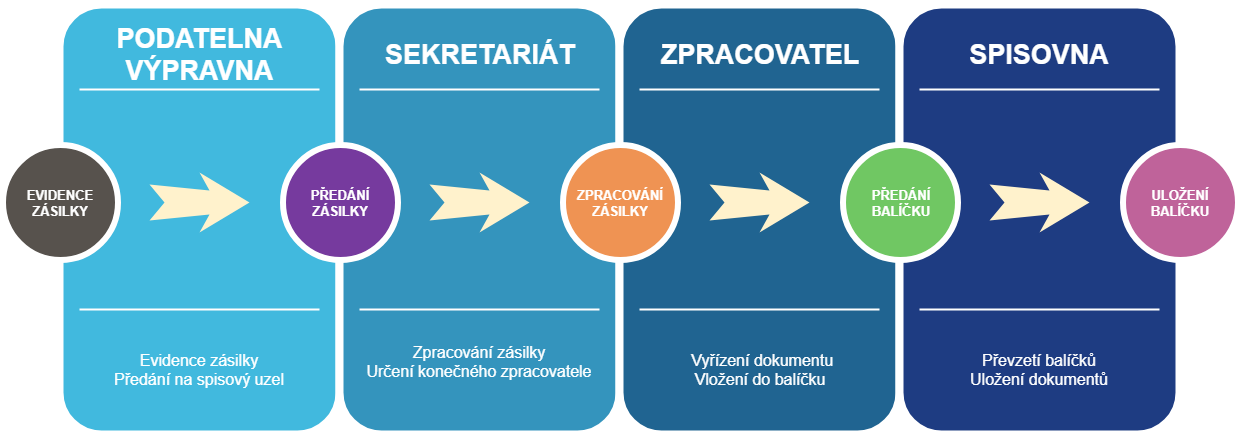
\includegraphics[width=0.9\linewidth]{./images/ERMSWorkflow1.png}} 
  \caption{Základní workflow.} 
\end{figure}

Aplikace ERMS je koncipována jako webová aplikace dostupná přes webové rozhraní (systém klient – server). Podporované jsou nejnovější verze prohlížečů Internet Explorer, Chrome a Firefox. Kompatibilní jsou i ostatní prohlížeče (např. Safari, Opera aj.).

Portál (založený na portálovém řešení Liferay CE) je dle funkcionality rozdělen do jednotlivých sekcí, které jsou přihlášenému uživateli nabízeny podle jemu přiřazených rolí. Administrace portálu, rozložení webu a správa statického obsahu je možná přímo přes administraci portálu. 

\subsection{Pojem ERMS}
Národní standard v roce 2016 zavedl pojem elektronický systém spisové služby (ERMS), který je převzatý z anglického Electronic Record Management System. V roce 2017 vychází nové vydání národního standardu a tam se používá pojem elektronická spisová služba (eSSL). V textu je pojem ERMS míněn jako konkrétní implementace eSSL firmy M.I.T. Consulting, s.r.o.
\newpage
\subsection{Hlavní funkce}
\begin{enumerate}
	\item Příjem a odesílání zásilek:
	\begin{itemize}
		\item Převzetí a odeslání zásilky klasickou a elektronickou poštou, nebo datovou schránkou.
		\item Elektronická podatelna.
		\item Evidence zásilek.
		\item Hromadná korespondence s~automatizovaným generováním ze šablony.
		\item Tisk poštovního podacího archu, poštovních zásilek a možnost napojení na frankovací stroj.
		\item Správa adresátů.
		\item Evidence doručenek, sledování zásilek pomocí Track\& Trace. 
	\end{itemize}
	\item Skenovací linka (s~desktopovou aplikací pro pracovníky skenovacích pracovišť).
	\item Správa dokumentů:
	\begin{itemize}
		\item Proces zpracování dokumentu od přijetí na podatelně, přes spisový uzel až po předání konkrétnímu zpracovateli.
		\item Možnost předávání zásilek mezi podatelnami.
		\item Zatřídění dokumentů do spisů, věcných skupin a sběrných archů.
		\item Evidence a uchovávání vlastních i doručených dokumentů v~digitální a analogové podobě. 
		\item Nastavení lhůty pro vyřízení dokumentu a její následná kontrola s~notifikacemi.
		\item Pokrytí komplexního životního cyklu dokumentu od podatelny po spisovnu a skartaci.
		\item Vytěžení a zaindexování všech atributů dokumentu.
		\item Vyhledávání a filtrování dokumentů podle všech atributů.
		\item Přístup k~uloženým dokumentům a jejich zobrazení.
	\end{itemize}
	\item Správa spisů:
	\begin{itemize}
		\item Schvalovací proces nad spisem.
		\item Definování oběhu spisů a požadavků na schvalování.
		\item Vkládání dokumentů do spisů.
		\item Propojení spisů s~dokumenty.
		\item Prolinkování s~jinými spisy a dokumenty.
	\end{itemize}
	\item Ukládání a skartace:
	\begin{itemize}
		\item Uložení uzavřených spisů a vyřízených dokumentů do spisovny.
		\item Tvorba spisového a skartačního plánu.
		\item Evidence a hlídání skartační lhůty.
		\item Proces skartace, skartační návrh, posuzování skartačních operací.
		\item Předání dokumentů do národního archivu.
		\item Zápůjčky.
		\item Automatizované převody vybraných typů elektronických dokumentů do archivního formátu PDF/A-2b.
		\item Zabezpečení dokumentu proti ztrátě, poškození nebo záměrnému podvržení v~datovém úložišti.
	\end{itemize}	
\end{enumerate}

\newpage
	\begin{figure}[h]
  \centerline{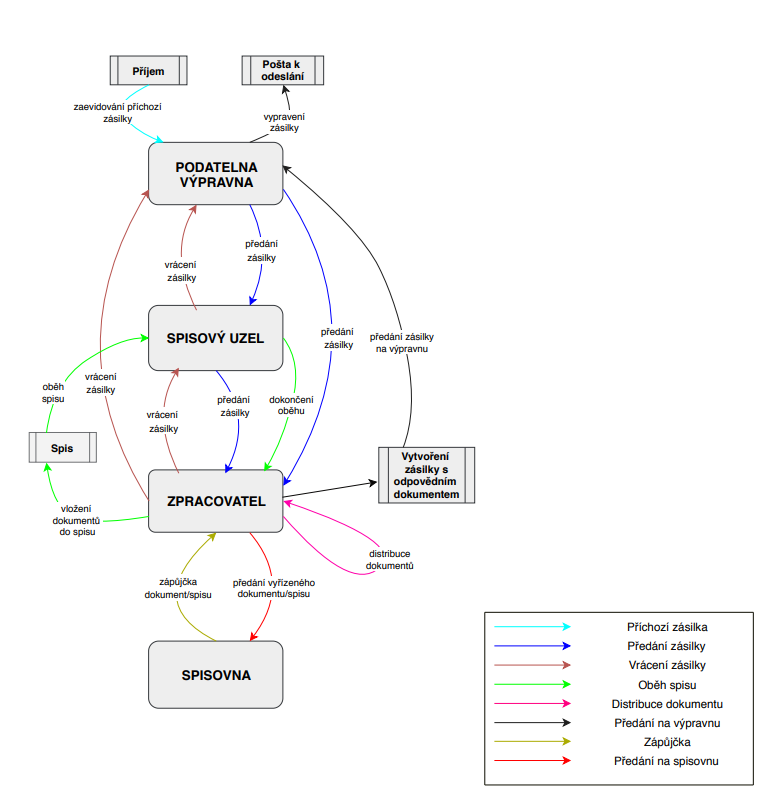
\includegraphics[width=1.1\linewidth]{./images/ERMSWorkflow2.png}} 
  \caption{Detail životního cyklu evidovaných entit.} 
\end{figure}


\newpage
\section{ISSD}

\newacronym{NSESSS}{NSESSS}{Národní standard pro elektronické systémy spisové služby dle §63 zákona č.499/2004 Sb.}
\newacronym{ISSD}{ISSD}{Informační systém spravující dokumenty}

\gls{NSESSS} zavedl pojem \gls{ISSD} pro systémy a agenty, které ERMS využívají pro tvorbu a správu dokumentů. Jedna z~nejvýznamnějších novinek čtvrté verze Národního standardu je standardizace rozhraní mezi elektronickým systémem spisové služby a ISSD. Toto rozhraní vychází z~dříve vydaných verzí tzv. Best practices\cite{o01} a reflektuje zkušenosti s~jeho implementací.

Rozhraní je řešeno na bázi webových služeb a obsahuje synchronní i asynchronní část\cite[s.~58]{o00}. Obě části se vzájemně doplňují, přičemž synchronní funkce se využívají pouze v~nezbytně nutné míře, protože jsou vždy závislé na aktuální dostupnosti obou provázaných systémů. Téměř veškerá komunikace, kromě okamžitého vyzvednutí čísla jednacího pro dokument nebo spisové značky pro spis, probíhá asynchronně, což znamená, že uživatelé jednoho systému mohou bez omezení pracovat, i když je druhý systém dočasně nedostupný.

V~rámci rozhraní je aplikován tzv. exkluzivní přístup k~entitám (výhradní správa). To znamená, že vždy jen jeden systém má aktuálně daný dokument či spis ve výhradní správě a může měnit jeho stav, popřípadě upravovat jeho popis, zatímco druhý systém je v~dané době pouze pasivním příjemcem informací o~těchto provedených událostech. Díky tomu, že data jsou vždy postupně synchronizována prostřednictvím jednotlivých událostí do obou komunikujících systémů, mají uživatelé obou systémů vždy přehled o~dokumentech a spisech.

Podle NSESSS je implementováno rozhraní pro zasílání notifikací systémům třetích stran. U~registrovaného systému se zjistí, jestli si systém přeje zasílat notifikace (možnost výběru během registrace) a v~pozitivním případě je zasílá na uvedený registrovaný endpoint s~použitím registrovaného přihlašovacího jména a hesla. 

ISSD systémy tvoří pomocnou evidenci dokumentů, přičemž se ERMS využívá jako centrální systém, ve kterém se udržují aktuální data. ERMS má díky implementaci všech metod synchronního a asynchronního rozhraní připravené prostředky tak, aby mohlo evidovat veškeré případné modifikace, ke kterým dochází během životního cyklu dané entity po dobu výhradní správy v~ISSD. Existuje několik způsobů jak se k~evidenci může přistupovat. Jeden z~případů nastává v~okamžiku, kdy je daný dokument nebo spis zaevidován v~ERMS. V~takovém případě výhradní správa ISSD nad entitou začíná notifikační událostí postoupení dokumentu nebo postoupení spisu.\footnote{Komunikace směrem z~ERMS do ISSD.} Touto notifikací se ISSD dozví všechna potřebná data, protože postoupení obsahuje profil dané entity.\footnote{Zejména přiřazené číslo jednací.} ISSD na své straně entitu zaeviduje a může začít vykonávat modifikační operace. Tyto modifikace jednotlivými voláními webových metod propaguje zpět do ERMS. Druhým případem je situace, kdy vznikne dokument nebo spis v~ISSD a ten voláním metody pro založení dokumentu nebo založení spisu zaeviduje entitu v~ERMS a tím se přiřadí číslo jednací. Entita zůstává ve výhradní správě ISSD a opět se pomocí webových metod synchronizují změny do ERMS. Životní cyklus výhradní správy v~ISSD končí předáním entity do výhradní správy ERMS. V~okamžiku, kdy se ukončuje celý životní cyklus entity a dojde ke skartačnímu řízení, odesílá se do ISSD notifikace o~tom, že se provedla skartace.\footnote{Aby ISSD mohl danou entitu označit jako skartovanou.}

\begin{table}
\begin{center}
\caption{Události povinně implementované na straně ISSD}\label{tab:IssdEvents}
\scalebox{0.95}{\begin{tabular}{>{\bfseries}l L{8cm}}
{\normalfont Název události} & {\normalfont Popis} \\
\hline

DokumentPostoupeni	&	Předání výhradní správy dokumentu. \\
SpisPostoupeni	&	Předání výhradní správy spisu. \\

VypraveniVypraveno	&	Předání informace o~vypravení zásilky. \\
VypraveniDoruceno	&	Předání informace o~doručení zásilky. \\
SouborZalozeni	&	Předání komponenty. \\
DokumentSkartovano	&	Předání informace o~proběhlém skartačním řízení dokumentu. \\
SpisSkartovano	&	Předání informace o~proběhlém skartačním řízení spisu. \\

\end{tabular}}
\end{center}
\end{table}

\subsection{Autentizace ISSD vůči ERMS}\label{ch:issd}

\newacronym{JAAS}{JAAS}{Java Authentication \& Authorization Service}

Pro autentizaci se využívá mechanismus HTML Basic Access Authentication.  Autentizaci na straně aplikace využívá modul, který je postaven na technologii \gls{JAAS}.\footnote{\url{https://docs.oracle.com/javase/6/docs/technotes/guides/security/jaas/JAASRefGuide.html}} Modul zaručuje, že ještě před samotným vykonáním metody, je volající systém zaregistrován, heslo je korektní a má příslušnou roli k~tomu, aby se požadovaná metoda mohla vykonat.

Uživatel s~rolí správce ERMS má možnost prostřednictvím webového rozhraní zaregistrovat systém ISSD a tím umožnit komunikaci (synchronní i asynchronní).

Pro novou registraci systému jsou potřeba následující parametry:
\begin{itemize}
	\item Kód systému -- max. 6 znaků.
	\item Název systému -- celé jméno systému.
	\item Uživatelské jméno systému -- slouží k~basic authentizaci jako username.
	\item Heslo -- slouží k~authentizaci jako password.
	\item Endpoint -- bude sloužit ke zpětnému volání.
	\item Notifikovat ISSD systém -- volba, jestli má být systém zpětně notifikován.
	\item ISSD uživatelské jméno -- autentizace ERMS vůči ISSD.
	\item ISSD heslo.
\end{itemize}

\begin{figure}[h]
  \centerline{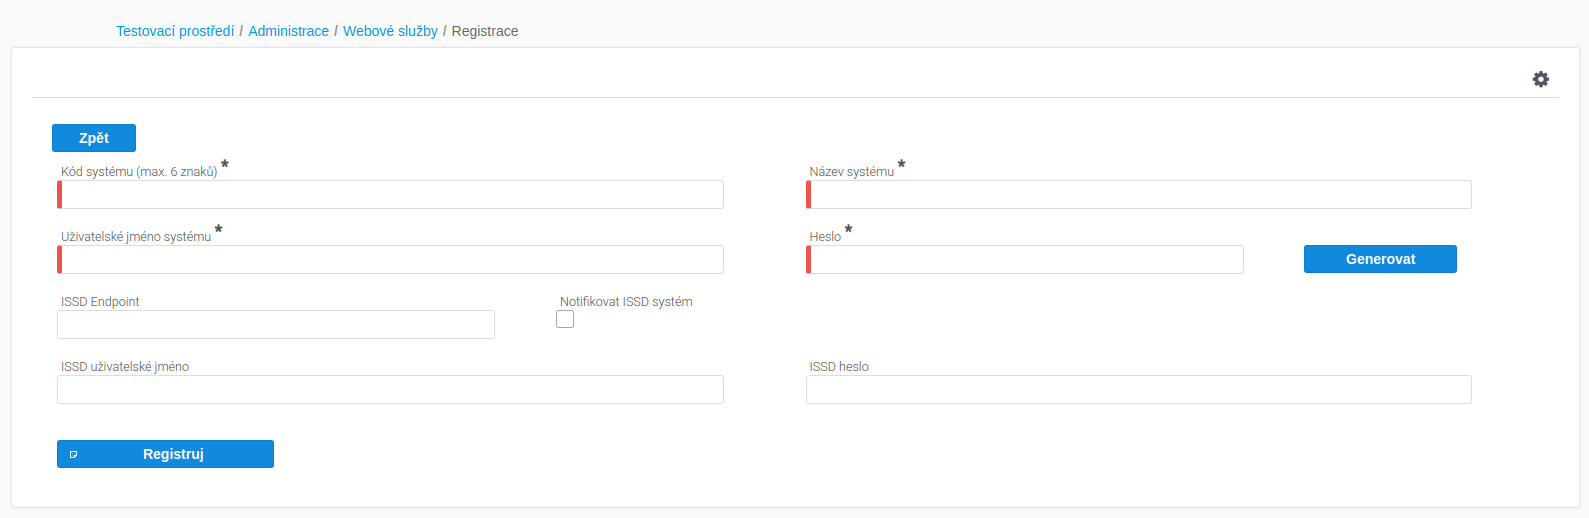
\includegraphics[width=0.9\linewidth]{./images/ISSDRegistration.png}} 
  \caption{Registrace nového ISSD klienta.} 
\end{figure}

Kód systému musí být v~rámci ERMS jednoznačný. Tento identifikátor se používá v~komunikaci v~atributu \kiinlinecode{text}{!}{zdroj} (v~případě příchozí komunikace) a nebo v~atributu \kiinlinecode{text}{!}{cil} (u~odchozí komunikace).

V~případě příchozí komunikace se ověří ISSD systém pomocí uživatelského jména a hesla systému. Toto je první fáze, kdy se kontroluje, jestli může volání projít dále do ERMS. Další fází je ověření zdroje a cíle. Zdroj se musí shodovat s~registrovaným kódem systému a cíl se musí shodovat s~kódem ERMS.\footnote{Požadavek 9.1.2 \cite[s.~59]{o00}.}

Název systému reprezentuje uživatelsky čitelné jméno, které se pak zpracovatelům prezentuje na webovém rozhraní.

Endpoint je adresa webových služeb vypublikovaná na straně ISSD systému. Tento endpoint slouží ke zpětnému volání ze strany ERMS, tzv. notifikace. Jedná se především o~notifikace postoupení dokumentu, spisu. Dále pak o~notifikace, kdy bylo vypravení vypraveno a doručeno. V~poslední řadě pak informace o~provedení skartace dokumentu či spisu. Všechny tyto notifikace slouží k~synchronizaci dat mezi ISSD a centrálním uzlem ERMS.

Endpoint ISSD systému může vyžadovat basic autentizaci. K~tomu slouží při registraci systému položky ISSD uživatelské jméno a ISSD heslo.

\subsection{Schéma komunikace}
ERMS hraje v~komunikaci roli centrálního uzlu (centrální evidence) a jednotlivé ISSD systémy komunikují s~jedním ERMS. Na základě definovaných principů NSESSS se počítá s~vzájemnou komunikací dvou systému, kde jedním z~nich je vždy ERMS. Vzájemná komunikace ISSD klientů není vyloučena, ale není standardem pokryta. 

ERMS komunikuje současně s~více ISSD. Proto je kladen důraz na striktní rozlišování, který ISSD komunikuje. Během komunikace se za účelem jednoznačnosti, kdo s~kým komunikuje, používá atributů ZDROJ a CIL. Tyto atributy jsou obsaženy v~každé XML zprávě. Jedná se o~řetězce identifikující oba komunikující systémy.

\newpage
\section{Princip synchronní a asynchronní komunikace}
Rozhraní je složeno ze dvou částí, které jsou implementovány současně a pracují nad společnými daty. Liší se jejich využití v~procesech organizace.

\subsection{Synchronní komunikace}
Pro požadavky, které vyžadují okamžitou odpověď, je definováno synchronní rozhraní webových služeb. Volání má formu request -- response. Odpovědní struktura vždy obsahuje výsledek volání (\kiinlinecode{text}{!}{OperaceStatus}). Pokud volání proběhlo v~pořádku, návratový kód je \kiinlinecode{text}{!}{0000} s~nepovinným popisem. Pokud během vykonávání dojde k~chybě, odpovědní struktura obsahuje chybový kód a stručný popis chyby.

\begin{figure}[h]
  \centerline{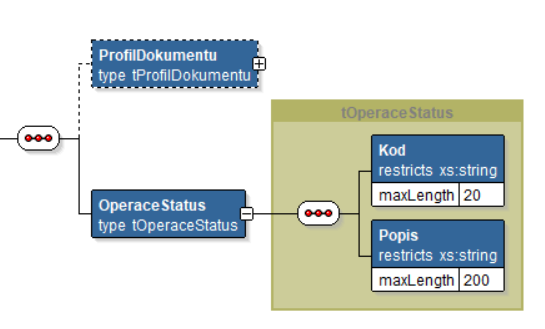
\includegraphics[width=0.9\linewidth]{./images/OperaceStatus.png}} 
  \caption{Návratová struktura s~výsledkem volání.} 
\end{figure}

Nejzásadnější volanou metodou je \kiinlinecode{text}{!}{DokumentZalozeni}, jelikož v~centrální evidenci (ERMS) vzniká dokument, kterému je přiřazené číslo jednací.

Speciální případ je metoda \kiinlinecode{text}{!}{Udalosti} sdružující více událostí, které se mají sekvenčně vykonat. Každá událost obsahuje atribut \kiinlinecode{text}{!}{UdalostId}, který zaručuje unikátnost události. Tento identifikátor je také použit pro spárování zprávy výsledku vykonání dané události.

\begin{figure}[h]
  \centerline{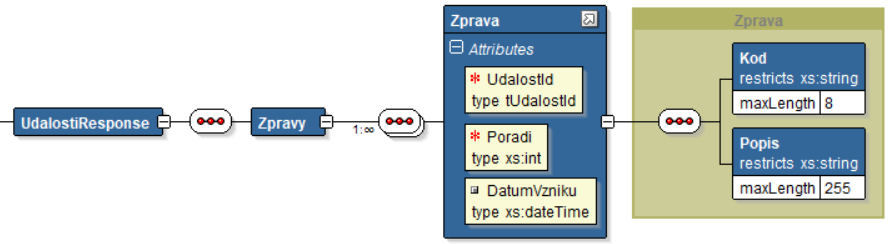
\includegraphics[width=0.9\linewidth]{./images/UdalostiResponse.png}} 
  \caption{Návratová struktura volání událostí.} 
\end{figure}

Volání uvažuje jednu transakci, ve které se vykonají všechny události. Znamená to, že pokud během sekvenčního vykonávání jednotlivých událostí dojde k~chybě, celá transakce je označená k~rollback, a tím pádem se nepovažuje ani žádná předchozí událost daného volání za vykonanou.

\begin{table}
\begin{center}
\caption{Metody synchronního rozhraní}\label{tab:ErmsSync}
\scalebox{0.95}{\begin{tabular}{>{\bfseries}l L{8cm}}
{\normalfont Název metody} & {\normalfont Popis} \\
\hline

DokumentZalozeni	&	Založení dokumentu, získání čísla jednacího. \\
SpisZalozeni	&	Založení spisu, získání spisové značky. \\
Udalosti	&	Žádost o~okamžité sekvenční vykonání předaného seznamu událostí. Vše v~jedné transakci. \\
DokumentPostoupeniZadost	&	Žádost o~předání výhradní správy dané entity z~ERMS do ISSD. \\
ProfilDokumentuZadost	&	Žádost o~poskytnutí detailních informací o~dokumentu. \\
ProfilSpisuZadost	&	Žádost o~poskytnutí detalních informací o~spisu. \\
SouborZadost	&	Žádost o~binární obsah komponenty. \\
CiselnikZadost	&	Žádost o~poskytnutí číselníku. \\
FunkcniMista	&	Žádost o~seznam organizačních součástí původce na základě osobního čísla uživatele. \\
DavkySeznam	&	Žádost o~seznam připravených, nepotvrzených dávek, které ERMS pro daný ISSD registruje. \\
DavkaZadost	&	Žádost o~zaslání konkrétní registrované dávky v~ERMS pro daný ISSD. \\

\end{tabular}}
\end{center}
\end{table}

Příkladem volání událostí je vypravení zásilky. V~první události dochází k~založení zásilky, ve druhé události se vytvořená zásilka předává na výpravnu. Pokud se jedná o~digitální vypravení, které nepodléhá schvalování a neúspěšně se pokusí automaticky vypravit,\footnote{Digitální vypravení zásilky se uvažuje prostřednictvím e-mailu nebo prostřednictvím datové schránky.} dojde k~rollback celého volání a zásilka nezůstane vytvořená. V~návratové struktuře je pak k~dané události připojena zpráva s~informací, že se vypravení nepodařilo.
V~takovém případě se považuje za vhodnější použití asynchronní komunikace, kde se transakce uvažují v~rámci jednotlivých událostí (není chtěné, aby neúspěšný pokus vypravení zásilky měl za následek nezaevidování zásilky v~systému).

\subsection{Příklad synchronní komunikace}
Uvažujme případ, kdy v~ISSD vznikne nový dokument. Tuto informaci potřebuje propagovat do ERMS, a tak zavolá meotdu \kiinlinecode{text}{!}{DokumentZalozeni}. Toto volání je synchronní, protože vyžaduje okamžitou odpověď, ve které se nachází přiřazené číslo jednací, se kterým ISSD dále potřebuje pracovat. Například k~vytvořenému dokumentu potřebuje vygenerovat PDF komponentu, kde v~textu uvádí číslo jednací nebo další informace, které získá až na základě výsledku volání.


\subsection{Asynchronní komunikace}
\begin{table}
\begin{center}
\caption{Metody asynchronního rozhraní}\label{tab:ErmsAsync}
\scalebox{0.95}{\begin{tabular}{>{\bfseries}l L{8cm}}
{\normalfont Název metody} & {\normalfont Popis} \\
\hline

ErmsAsyn	&	Přenos dávek obsahující události a zprávy.\footnote{podle NSESSS 9.1.9.} \\
WsTest	&	Funkce pro ověření dostupnosti ERMS nebo ISSD. \\

\end{tabular}}
\end{center}
\end{table}

Synchronní komunikace je vhodná pro volání metod, na které uživatel očekává okamžitou odpověď. Asynchronní komunikace je složitější a dochází k~mnoha prodlevám. Typické využití spočívá v~tom, že se na jedné straně nahromadí fronta požadavků, které jsou periodicky vyzvednuty, seskládány do dávky a vytvořená dávka je následně odeslána protistraně pomocí komunikačního kanálu. Odeslání dávky spočívá ve volání metody \kiinlinecode{text}{!}{ErmsAsyn} na endpoint webové služby, která běží na straně cílového systému.

Příjemce dávky kontroluje její formální správnost a pak ji uloží pro následné zpracování. Formální kontrola dávky probíhá následovně:\footnote{Požadavky 9.1.13 až 9.1.24 \cite[s.~63--64]{o00}}
\begin{itemize}\label{enum:prichoziDavka}
	\item Zaslaná dávka musí navazovat na předchozí jak pořadím (1,2,3,4,...), tak datem vzniku.
	\item Žádná dávka nesmí byt ve stavu \kiinlinecode{text}{!}{ERROR}. Jestliže ERMS některou z~předchozích dávek zpracoval do stavu \kiinlinecode{text}{!}{ERROR}, systém čeká na opravnou dávku se stejným pořadím. Jakmile je zaslána opravná dávka, systém smaže všechny dříve zaslané dávky s~vyšším pořadím, než je dávka opravná.
	\item Zdroj dávky musí být registrovaný ISSD klient.
	\item Id událostí dávky musí být unikátní.
\end{itemize}
 
Obsah uložené dávky se zpracuje a během tohoto procesu vznikají zprávy odpovídající na zpracovávané události. Tyto zprávy se poskládají do dávky a jsou odeslány protistraně, která zprávy opět odloženě zpracuje a teprve po potvrzení úspěšného přijetí a zpracování událostí může být dávka považována za převzatou a zpracovanou protistranou.\footnote{Požadavek 9.1.23 \cite[s.~64]{o00}.}

\begin{figure}[h]
  \centerline{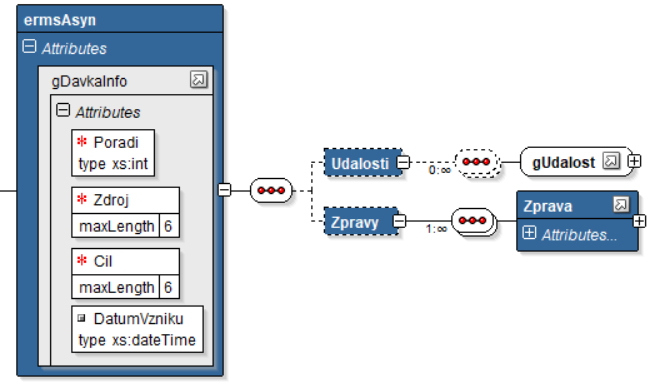
\includegraphics[width=0.9\linewidth]{./images/ErmsAsyn.png}} 
  \caption{Struktura ErmsAsyn.} 
\end{figure}

Pro dávkovou komunikaci je použita metoda \kiinlinecode{text}{!}{ErmsAsyn} obsahující následující atributy:
\begin{itemize}
	\item \kiinlinecode{text}{!}{Udalosti}: obsahuje seznam událostí, které v~rámci dávky budou zpracovány. Každá událost musí mít jednoznačný identifikátor v~rámci jedné dávky. Události se vykonávají dle atributu udalostId od nejmenšího po největší. 
	\item \kiinlinecode{text}{!}{Zpravy}: obsahuje seznam zpráv, které jsou vázané na udalostId, kód \kiinlinecode{text}{!}{0000} znamená, že událost byla korektně provedena. V~případě chyby návratový kód obsahuje i popis chyby. Jestliže je událost provedena korektně, popis nemusí být obsažen.
	\item \kiinlinecode{text}{!}{Poradi}: celková neklesající spojitá posloupnost zpracování dávek. Dávky jsou číslovány od 1 s~přírůstkem +1.
	\item \kiinlinecode{text}{!}{Zdroj}: identifikace volajícího systému.
	\item \kiinlinecode{text}{!}{Cil}: identifikace volaného systému.
	\item \kiinlinecode{text}{!}{DatumVzniku}: systém ERMS kontroluje před uložením dávky, zda příchozí dávka má novější datum, než poslední uložená, na kterou tato dávka bude navazovat.
\end{itemize}

\subsubsection{Evidence příchozích dávek v~ERMS}
Proces přijetí příchozí dávky splňuje všechny formální body \ref{enum:prichoziDavka}. Pokud některá podmínka přijetí dávky není splněná, volání vrací \kiinlinecode{text}{!}{SOAPException} a dávka není uložena ke zpracování. V~opačném případě se ukládá k~odloženému zpracování.

\begin{figure}[h]\label{im:prichoziDavka}
  \centerline{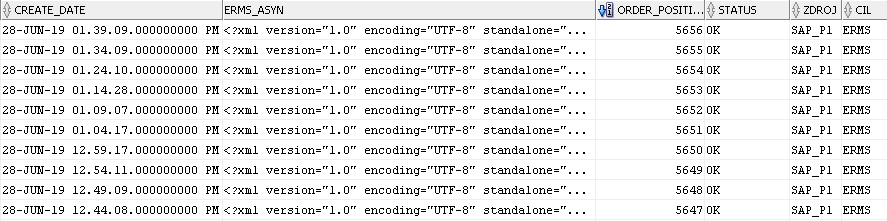
\includegraphics[width=0.9\linewidth]{./images/IncommingBatch.png}} 
  \caption{Evidence příchozích dávek.} 
\end{figure}

Na obrázku \ref{im:prichoziDavka} jsou vidět klíčové atributy evidované příchozí dávky:
\begin{itemize}
	\item Datum vzniku dávky.
	\item Obsah dávky.
	\item Pořadí dávky.
	\item Stav zpracování dávky.
	\item Zdroj (identifikátor ISSD).
	\item Cíl.
\end{itemize}

Atribut \kiinlinecode{text}{!}{STATUS} má následující životní cyklus:
\begin{itemize}
	\item \kiinlinecode{text}{!}{WAIT}: formálně přijatá dávka čekající na zpracování.
	\item \kiinlinecode{text}{!}{INPROCESS}: aktuálně zpracovávaná dávka.
	\item \kiinlinecode{text}{!}{ERROR}: dávka, jejíž vykonávání skončilo chybou.
	\item \kiinlinecode{text}{!}{FIXED}: přijatá opravná dávka, kterou lze vykonat.
	\item \kiinlinecode{text}{!}{OK}: úspěšně vykonaná dávka.     
\end{itemize}

CRONem spouštěná metoda se stará o~odložené vykonávání uložených dávek. Dochází ke kontrole, jestli není některá dávka ve fázi vykonávání (\kiinlinecode{text}{!}{INPROCESS}) nebo ve stavu \kiinlinecode{text}{!}{ERROR} a pokud ne, vybere nejnižší pořadí dávky se stavem \kiinlinecode{text}{!}{WAIT} nebo \kiinlinecode{text}{!}{FIXED} a tu začne vykonávat. Během zpracování se pro jednotlivé události generují odpovědní zprávy, které se ukládají pro odložené odeslání protistraně.


\subsubsection{Mechanismus tvoření odchozích dávek v~ERMS}
Tvorba odchozích dávek je rozdělena na dvě části. Obě se vykonávají v~pravidelných intervalech.
\begin{enumerate}
	\item Proces tvorby odchozí dávky.\\
	Tvorba odchozí dávky se provádí v~nové transakci pro každý registrovaný ISSD, a to z~toho důvodu, aby komunikace byla striktně izolovaná a případný rollback sestavení odchozí dávky pro jeden systém nezablokoval komunikaci s~dalšími systémy. Události, které se mohou v~odchozí dávce vyskytovat, jsou definované požadavkem 9.1.12 \cite[s.~63]{o00} (tabulka \ref{tab:IssdEvents}).
	
	Životní cyklus odchozí události:
\begin{itemize}
	\item \kiinlinecode{text}{!}{NEW}: nová událost čekající na zpracování do odchozí dávky.
	\item \kiinlinecode{text}{!}{PREAPRED}: událost obsažená v~některé odchozí dávce, u~které ještě nedošlo k~formálnímu přijetí protistranou.
	\item \kiinlinecode{text}{!}{SENT}: odeslaná událost v~některé odchozí dávce.
	\item \kiinlinecode{text}{!}{OK}: potvrzené zpracování události protistranou.    
\end{itemize}
	
	Proces vezme všechny zprávy, které jsou evidované k~odeslání danému ISSD (zprávy ve stavu \kiinlinecode{text}{!}{NEW}).
	
	Dále se vezmou všechny události, které mají stav \kiinlinecode{text}{!}{NEW} pro daný ISSD.
	
	V~případě události \kiinlinecode{text}{!}{DokumentPostoupeni} nebo \kiinlinecode{text}{!}{SpisPostoupeni}, která obsahuje digitální dokument a k~němu připojené komponenty, dochází ke kontrole, zda byla u~komponent dokončena jejich transformace.\footnote{Transformace je proces definovaný národním standardem, který komponenty převádí do výstupního datového formátu. Viz kapitola 5.3 \cite[s.~39]{o00}.} Pokud ne, je událost v~aktuální iteraci přeskočena a do dávky se nepřidává.
	
	Vzniká nová odchozí dávka a všechny události a zprávy v~ní obsažené jsou označeny id dané dávky a přepnuty do stavu \kiinlinecode{text}{!}{PREPARED}.

\begin{figure}[h]
  \centerline{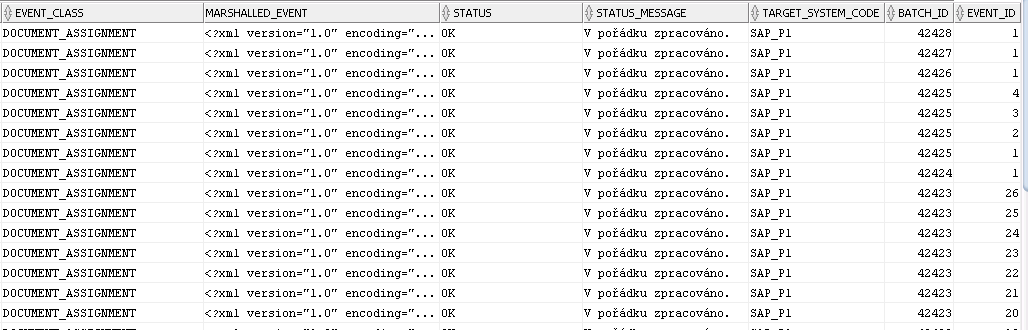
\includegraphics[width=0.9\linewidth]{./images/OutgoingBatchEvent.png}} 
  \caption{Evidence odchozích událostí.} 
\end{figure}

	\item Proces odeslání připravené odchozí dávky.\\	
	Životní cyklus odchozí dávky:
\begin{itemize}
	\item \kiinlinecode{text}{!}{NEW}: nová odchozí dávka čekající na odeslání.
	\item \kiinlinecode{text}{!}{ERROR}: neúspěšně doručená dávka.
	\item \kiinlinecode{text}{!}{SENT}: doručená dávka (formálně přijatá na straně ISSD).
	\item \kiinlinecode{text}{!}{OK}: potvrzené zpracování protistranou.    
\end{itemize}

	Proces vykonává pokus o~odeslání dávky v~nové transakci pro každý registrovaný ISSD.
	
	Vybere se dávka s~nejnižším pořadím se stavem 	\kiinlinecode{text}{!}{NEW} nebo \kiinlinecode{text}{!}{ERROR} a provede se pokus o~její odeslání.
	
	Pokud je dávka na straně ISSD formálně přijata, označí se stavem \kiinlinecode{text}{!}{SENT} a provede se aktualizace stavů zpráv a událostí v~ní obsažených.	

\begin{figure}[h]
  \centerline{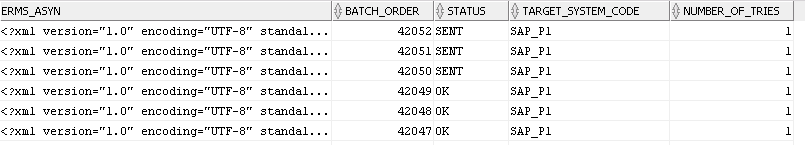
\includegraphics[width=0.9\linewidth]{./images/OutgoingBatch.png}} 
  \caption{Evidence odchozích dávek.} 
\end{figure}
\end{enumerate}

\subsection{Příklad asynchronní komunikace}
Uvažujme scénář, kdy dokument vznikne na straně ERMS. Následující kroky využívající asynchronní (i synchronní) komunikaci můžou vypadat následovně:\footnote{V závorce je uvedený název volané metody.}

\begin{enumerate}
	\item ERMS vytvoří notifikaci o~postoupení dokumentu do ISSD. (ErmsAsyn)
	\item ISSD dávku zpracuje a odesílá potvrzující zprávu. (ErmsAsyn)
	\item ISSD zakládá spis. (SpisZalozeniRequest)
	\item ISSD vytváří dávku (ErmsAsyn) sdružující události:
	\begin{itemize}
		\item Založení komponenty. (SouborZalozeni)
		\item Připojení komponenty k~dokumentu. (SouborVlozitKDokumentu)
		\item Zatřízení dokumentu do spisu. (DokumentVlozeniDoSpisu)
		\item Vytvoření odchozí zásilky. (VypraveniZalozeni)
		\item Vypravení zásilky. (VypraveniPredatVypravne)
		\item Vyřízení spisu. (SpisVyrizeni).
		\item Uzavření spisu. (SpisUzavreni).
		\item Předání spisu do výhradní správy ERMS. (SpisVraceni).
	\end{itemize}
	\item ERMS dávku zpracuje a odesílá potvrzující zprávy. (ErmsAsyn)
\end{enumerate}

Jak je vidět, asynchronní proces je rozdělený na několik fází, a tak úkony trvají podstatně delší dobu než v~případě synchronní komunikace. Výhodou je však větší robustnost a princip transakcí uvažovaný v~rámci jednotlivých událostí. Dojde-li k~chybě, nemusí celý proces začínat od začátku, ale pouze se komunikace obnoví opravnou dávkou, která začíná až tou událostí, kde došlo k~chybě.


\newpage
\section{Popis struktur a význam jednotlivých vnořených částí}
Následující kapitola popisuje chování jednotlivých metod rozhraní.

\subsection{Společné vnořené struktury}
\begin{figure}[h]
  \centerline{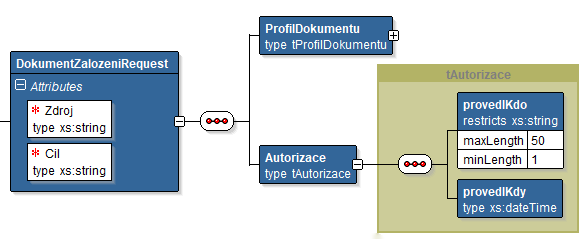
\includegraphics[width=0.9\linewidth]{./images/Autorizace.png}} 
  \caption{Struktura autorizace.} 
\end{figure}
Pro všechna volání je struktura \kiinlinecode{text}{!}{Autorizace} shodná. Atribut \kiinlinecode{text}{!}{ProvedlKdo} obsahuje identifikátor daného uživatele. Na začátku volání každé metody se provádí autorizace na základě předané hodnoty. Pokud uživatel existuje, provádí se metoda jeho jménem. V~opačném případě je chyba ohlášena návratovým kódem.

Atributy obsahující datum musí být ve formátu \kiinlinecode{text}{!}{yyyy-MM-dd'T'HH:mm:ss'Z'} (příklad 2018-04-11T12:25:42.578+02:00)

V~okamžiku odeslání požadavku přes SOAP dochází k~validaci a ověřuje se, zda jsou vyplněné všechny povinné údaje. Pokud ne, oznámí se uživateli, která položka chybí. V~některých případech je pro správné fungování ERMS vyžadováno vyplnění některých nepovinných atributů a v~průběhu vykonávání metody se kontroluje, jestli jsou uvedené a jestli mají správný formát a obsah.

Identifikátor je v~režii jednotlivých ISSD. Obsahuje atributy \kiinlinecode{text}{!}{Hodnota} a \kiinlinecode{text}{!}{Zdroj}. Kombinace těchto atributů musí být unikátní napříč celým systémem.

\subsection{Založení dokumentu}
\begin{figure}[h]
  \centerline{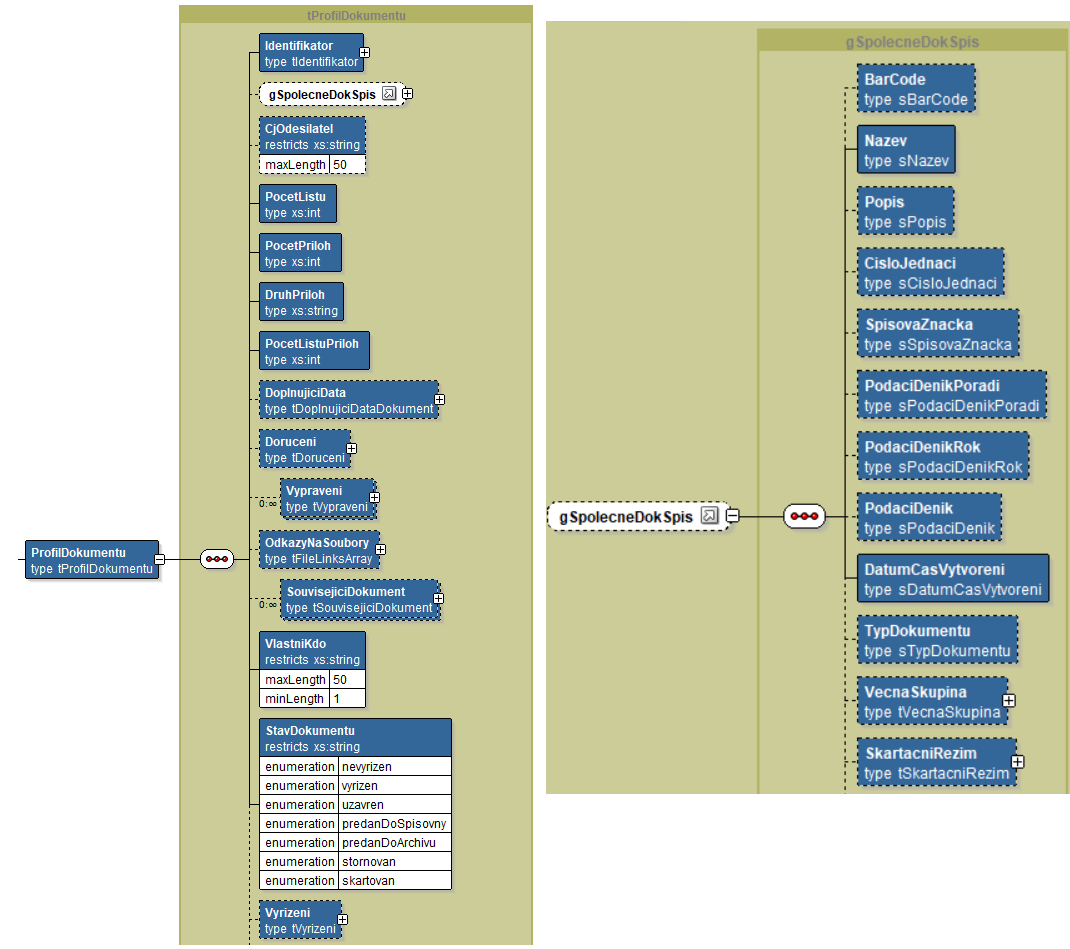
\includegraphics[width=0.9\linewidth]{./images/ProfilDokumentu.png}} 
  \caption{Struktura profilu dokumentu.} 
\end{figure}

Struktura profilu dokumentu je společná pro více volání, a proto jsou během zakládání dokumentu některé atributy zbytečné, až matoucí.

Nejjednodušší struktura je pro založení digitálního nevyřízeného vlastního dokumentu bez komponent:
\begin{itemize}
	\item \kiinlinecode{text}{!}{Identifikator}: jednoznačný identifikátor dokumentu.
	\item \kiinlinecode{text}{!}{Nazev}: Název dokumentu -- věc.
	\item \kiinlinecode{text}{!}{DatumCasVytvoreni}.
	\item \kiinlinecode{text}{!}{PocetListu}.
	\item \kiinlinecode{text}{!}{DruhPriloh}.
	\item \kiinlinecode{text}{!}{VlastnilKdo}: identifikátor zpracovatele, kterému se má zakládaný dokument přiřadit.
	\item \kiinlinecode{text}{!}{StavDokumentu}: základní stav je \kiinlinecode{text}{!}{nevyrizen}.
\end{itemize}

V~atributu \kiinlinecode{text}{!}{VecnaSkupina} se předává identifikátor věcné skupiny, do které má být dokument zatřízen. Pokud není vyplněný atribut \kiinlinecode{text}{!}{TypDokumentu}, je vybrán výchozí typ dokumentu. Bude-li atribut vyplněn, ale daný typ dokumentu nebude nalezen v~databázi, dochází k~chybě. Typ dokumentu se určuje pomocí identifikátoru, který lze získat pomocí číselníku.

Založený dokument musí být zatřízen, a proto jeden z~atributů \kiinlinecode{text}{!}{VecnaSkupina} nebo \kiinlinecode{text}{!}{SpisovaZnacka} musí být vyplněn.

Struktura \kiinlinecode{text}{!}{SkartacniRezim} je úzce vázána na spisový plán a věcnou skupinu, tudíž se bere z~ní a zde není uvažována.

Vlastnictví dokumentu se odvozuje od uživatele ze struktury \kiinlinecode{text}{!}{ProvedlKdo} výběrem nejbližší organizační jednotky s~vyplněným údajem \kiinlinecode{text}{!}{IdERMS}.

Změnou hodnoty \kiinlinecode{text}{!}{StavDokumentu} je možné modifikovat, jaký dokument se má vytvořit. V~závislosti na hodnotě vyplývají povinné doplňující struktury:

\subsubsection{Vyřízený dokument}      
\begin{figure}[h]
  \centerline{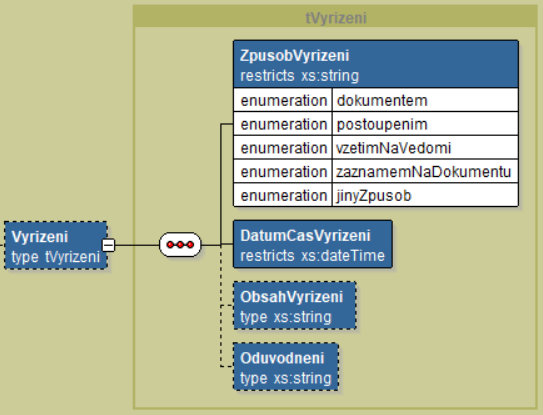
\includegraphics[width=0.9\linewidth]{./images/Vyrizeni.png}} 
  \caption{Struktura vyřízení.} 
\end{figure}         
               
V~případě stavu dokumentu s~hodnotou \kiinlinecode{text}{!}{vyrizen} je nutné vyplnit strukturu \kiinlinecode{text}{!}{Vyrizeni}, která obsahuje způsob vyřízení, datum vyřízení, obsah vyřízení a odůvodnění. Povinnost atributů je stejná, jako při běženém vyřizování dokumentu. Pokud jde o~jiný způsob, je obsah a odůvodnění vyžadováno.

V~případě zakládání dokumentu vyřízeného dokumentem chybí v~základních atributech možnost předávat identifikátor vyřizujícího dokumentu. Proto se musí využít struktura \kiinlinecode{text}{!}{DoplnujiciData} v~profilu dokumentu pomocí rozšiřujícího elementu \kiinlinecode{text}{!}{VyrizujiciDokument}.

\subsubsection{Uzavřený dokument}
Stavu dokumentu s~hodnotou \kiinlinecode{text}{!}{uzavren} a vyplněná struktura \kiinlinecode{text}{!}{DatumCasUzavreni}. 

\subsubsection{Digitální dokument s~komponentami}   
\begin{figure}[h]
  \centerline{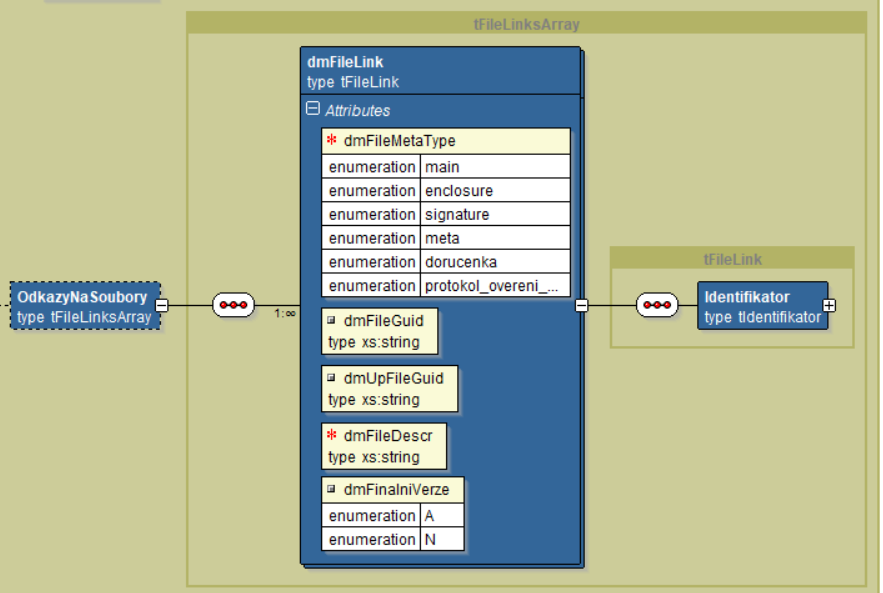
\includegraphics[width=0.9\linewidth]{./images/OdkazyNaSoubory.png}} 
  \caption{Struktura komponent.} 
\end{figure}         
Pro založení digitálního dokumentu s~připojenými komponentami je nutné, aby byla vyplněná struktura \kiinlinecode{text}{!}{OdkazyNaSoubory} obsahující seznam komponent, které mají být k~dokumentu připojeny. Atribut \kiinlinecode{text}{!}{dmFileMetaType} určuje vztah komponenty vůči dokumentu. Typ \kiinlinecode{text}{!}{main} může mít jen jedna komponenta, další komponenty bývají přílohy a pro ty se volí hodnota \kiinlinecode{text}{!}{enclosure}. Název souboru včetně přípony se uvádí v~atributu \kiinlinecode{text}{!}{dmFileDescr}.

\subsubsection{Doručený dokument}  
\begin{figure}[h]
  \centerline{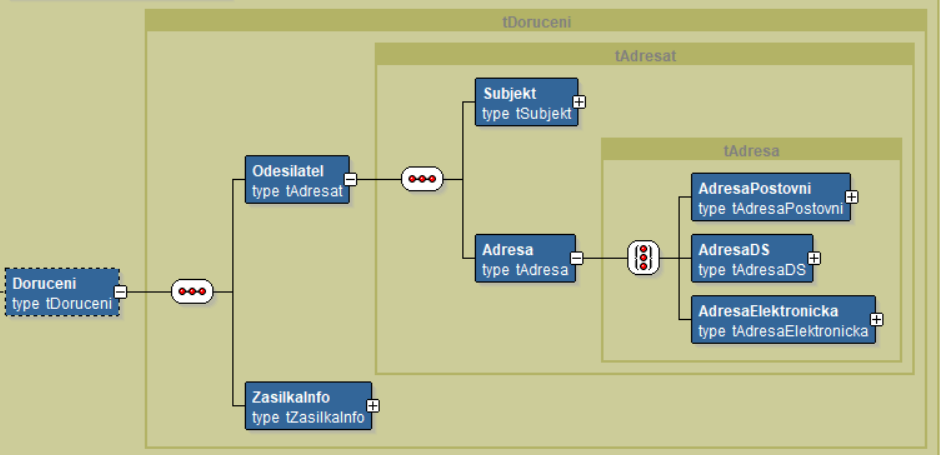
\includegraphics[width=0.9\linewidth]{./images/Doruceni.png}} 
  \caption{Struktura informací o~doručení.} 
\end{figure}            
Vznik doručeného dokumentu přes webové služby simuluje evidenci přijaté zásilky v~ISSD a její synchronizace do spisové služby. V~ERMS by se jednalo o~workflow přijetí zásilky na podatelně, její zaevidování a předání přes sekretariát až k~určenému zpracovateli. V~případě zakládání takového dokumentu se musí vyplnit struktura \kiinlinecode{text}{!}{Vypraveni}. Jedná se o~nejkomplexnější strukturu profilu dokumentu.

\kiinlinecode{text}{!}{Subjekt} obsahuje informace o~odesílateli. Zásadní je atribut \kiinlinecode{text}{!}{TypSubjektu}, který určuje, jestli je odesílatel právnická nebo fyzická osoba. V~závislosti na typu subjektu se pak vyplňují atributy jméno a příjmení, či obchodní název.

\kiinlinecode{text}{!}{Adresa} určuje způsob, jakým byl dokument doručen. Základní dělení je poštou, datovou schránkou, nebo elektronicky (e-mailem). Nutno vyplnit pouze jednu z~možností. V~závislosti na typu adresy se vyplňují další atributy ve struktuře \kiinlinecode{text}{!}{ZasilkaInfo}.

Způsob doručení se určuje strukturou \kiinlinecode{text}{!}{ZpusobManipulaceId} a pro doručený dokument může nabývat hodnot Posta, Osobne, ElektronickaPosta, EPodatelnaWeb, nebo DatovaSchranka, což jsou v~ERMS validní způsoby doručení. V~opačném případě je uživateli oznámena chyba, že se jedná o~neznámý typ doručení. Dále se ještě uvádí datum doručení.

\subsubsection{Dokument ve spisu}           
Při vytváření dokumentu je možné zvolit případ, kdy se vytvářený dokument zatřídí do existujícího spisu. Toto lze učinit vyplněním atributu \kiinlinecode{text}{!}{SpisovaZnacka}, který pak musí obsahovat identifikátor spisu. Struktura \kiinlinecode{text}{!}{VecnaSkupina} se pak neuvádí.

\subsection{Aktualizce dokumentu}
Pokud v~ISSD dojde ke změně některých informací týkajících se dokumentu, musí se tyto změny synchronizovat do ERMS prostřednictvím volání metody \kiinlinecode{text}{!}{DokumentUprava}. Ne všechny atributy, které obsahuje profil dokumentu je možné automaticky aktualizovat, protože by mohlo dojít k~nekonzistenci.
Atributy, které lze měnit:
\begin{itemize}
	\item Nazev (nesmí být null).
	\item BarCode.
	\item Popis.
	\item DatumCasVytvoreni.
	\item Poznamka (přidání nové poznámky, původní je nezměněna).
	\item Zmocneni.
	\item PocetListu.
	\item PocetPriloh.
	\item PocetListuPriloh.
	\item DruhPriloh.
\end{itemize}

\subsection{Vrácení dokumentu (předání do ERMS)}  
\begin{figure}[h]
  \centerline{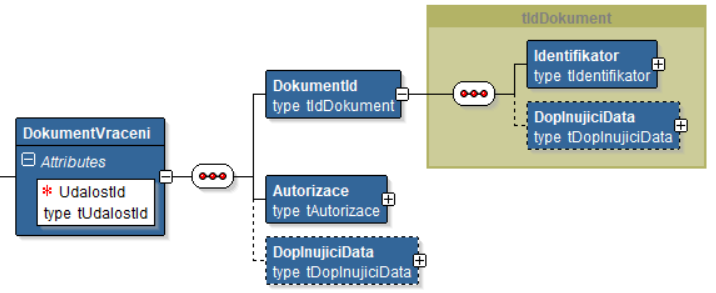
\includegraphics[width=0.9\linewidth]{./images/DokumentVraceni.png}} 
  \caption{Struktura vrácení výhradní správy dokumentu.} 
\end{figure}  
V~okamžiku, kdy ISSD přestává manipulovat s~dokumentem, předává výhradní správu zpět ERMS, aby bylo možné dokument uložit na spisovnu a v~určenou dobu zahájit skartační řízení.

\subsection{Stornování dokumentu}   
\begin{figure}[h]
  \centerline{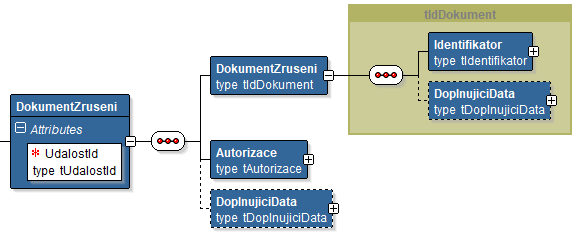
\includegraphics[width=0.9\linewidth]{./images/UdalostDokumentStorno.png}} 
  \caption{Struktura stornování dokumentu.} 
\end{figure}  
Stornování dokumentu se provádí pomocí události \kiinlinecode{text}{!}{DokumentZruseni}. V~takovém případě se připojuje automatické odůvodnění, že dokument byl stornován systémem. 


\subsection{Založení spisu}
\begin{figure}[h]
  \centerline{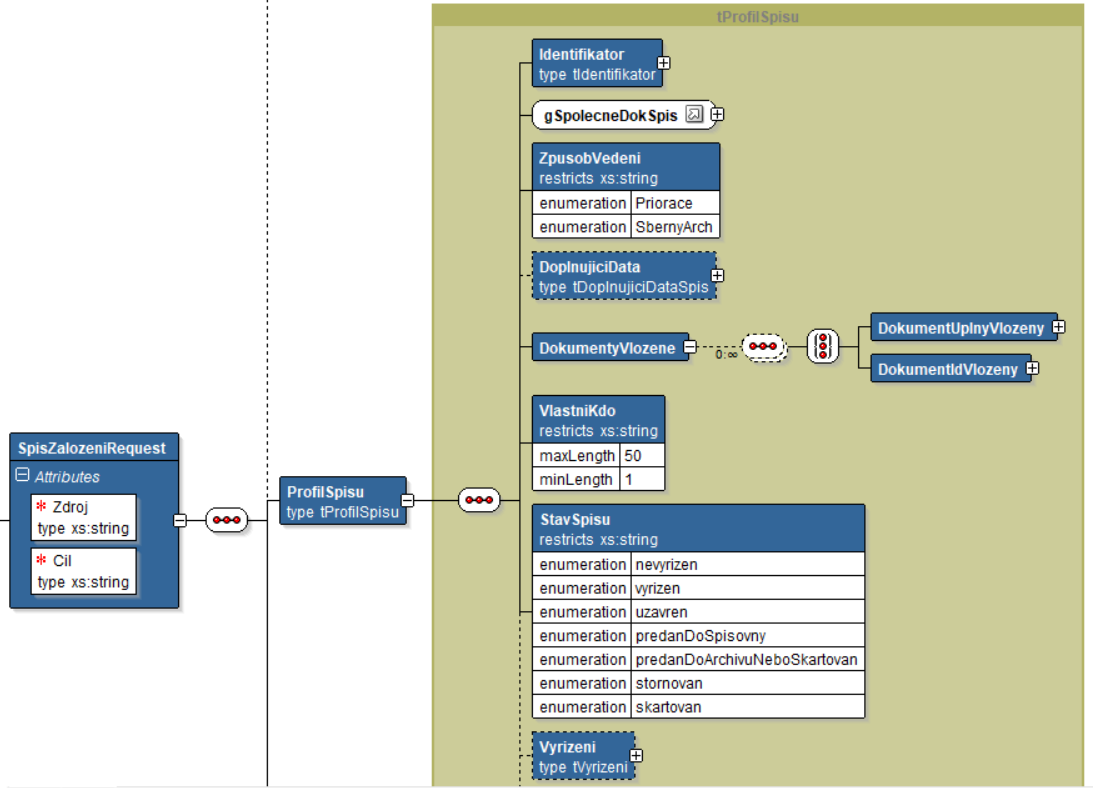
\includegraphics[width=0.9\linewidth]{./images/SpisZalozeni.png}} 
  \caption{Struktura založení spisu.} 
\end{figure} 

Většina atributů je shodných jako v~případě zakládání dokumentu. Navíc se v~profilu spisu vyskytuje atribut \kiinlinecode{text}{!}{ZpusobVedeni}, který určuje, jestli se jedná o~klasický spis, nebo o~sběrný arch. V~případě běžného spisu je umožněno založení prázdného spisu bez vloženého dokumentu (nebo dokumentů). V~případě sběrného archu je vyžadován minimálně jeden dokument (iniciační dokument sběrného archu).

Pokud se do spisu má rovnou zatřídit nějaký dokument, existují dva způsoby:

\subsubsection{Založení spisu s~odkazem na dokument}   
Struktura \kiinlinecode{text}{!}{DokumentyVlozene} obsahuje seznam dokumentů pouze odkazem na existující evidované dokumenty v~ERMS, které jsou ve výhradní správě daného ISSD. V~takovém případě se dokumenty určují prostřednictvím struktury \kiinlinecode{text}{!}{DokumentIdVlozeny} a dochází k~jejich zatřízení do vznikajícího spisu.

\subsubsection{Založení spisu s~úplným profilem dokumentu}
V~případě, že se během procesu zakládání spisu mají zaevidovat dokumenty, které nejsou v~ERMS evidované, využije se struktura \kiinlinecode{text}{!}{DokumentUplnyVlozeny}.

\subsection{Založení vyřízeného spisu}
Jedná se o~stejný princip jako v~případě dokumentu (vyplněná struktura \kiinlinecode{text}{!}{Vyrizeni} a stav spisu nastaven na \kiinlinecode{text}{!}{vyrizen}).

\subsection{Vyřízení spisu}
Událost má název \kiinlinecode{text}{!}{SpisVyrizeni} a jedná se o~shodnou strukturu jako v~případě, kdy se zakládá vyřízený spis.

\subsection{Uzavření spisu}  
V~ERMS existuje možnost vyřízení spisu jeho uzavřením. Pro volání webových služeb jsou toto dva oddělené kroky, a proto se po vyřízení spisu musí zavolat událost \kiinlinecode{text}{!}{SpisUzavreni}, aby se docílilo stejného stavu jako při shodné operaci v~ERMS.

\subsection{Vrácení spisu (předání do ERMS)}         
Stejný princip jako při vracení výhradní správy dokumentu.

\subsection{Stornování spisu}     
Stejný princip jako při stornování dokumentu.

\subsection{Manipulace s~dokumenty ve spisu}
Pomocí volání událostí \kiinlinecode{text}{!}{DokumentVlozeniDoSpisu} a \kiinlinecode{text}{!}{DokumentVyjmoutZeSpisu} lze dané dokumenty zatřídit do spisu a nebo je ze spisu vytřídit.

\subsection{Vytváření komponent}
\begin{figure}[h]
  \centerline{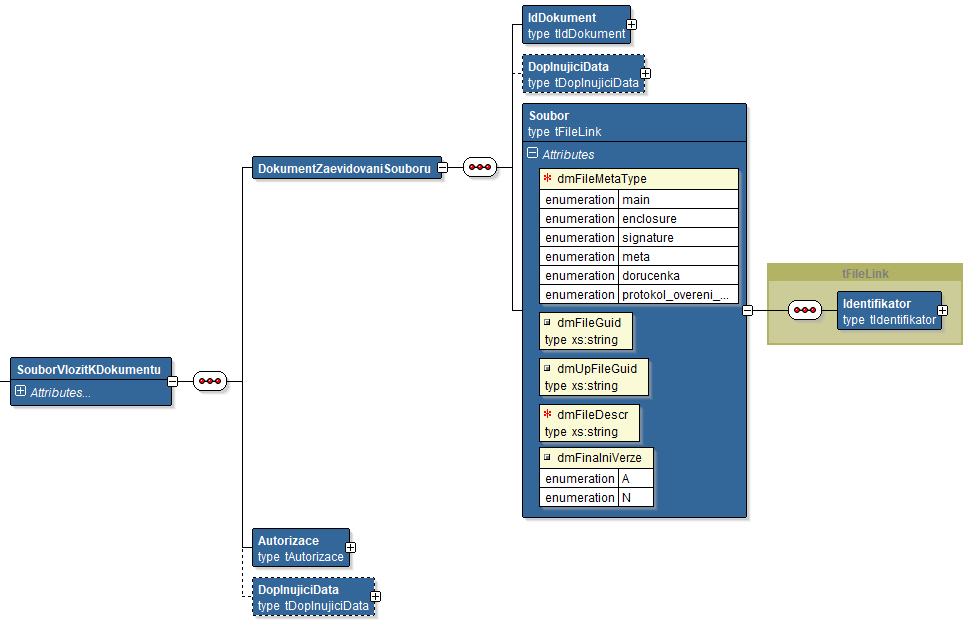
\includegraphics[width=0.9\linewidth]{./images/UdalostSouborVlozitKDokumentu.png}} 
  \caption{Připojení existující komponenty k~existujícímu dokumentu.} 
\end{figure} 
Obsah komponent je ve struktuře zakódovaný pomocí Base64. Vzniklý soubor pomocí události \kiinlinecode{text}{!}{SouborZalozeni} existuje bez vazby na dokument. Připojení komponenty k~dokumentu může proběhnout dvěma způsoby:
\begin{enumerate}
	\item Během zakládání dokumentu pomocí struktury \kiinlinecode{text}{!}{OdkazyNaSoubory}.
	\item Voláním události \kiinlinecode{text}{!}{SouborVlozitKDokumentu}.
\end{enumerate}
V~obou případech musí být komponenty založeny daným ISSD a v~případě připojování komponenty k~existujícímu dokumentu musí být i daný dokument ve výhradní správe ISSD.

\subsection{Události}
\begin{figure}[h]
  \centerline{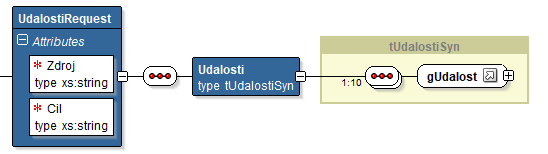
\includegraphics[width=0.9\linewidth]{./images/UdalostiRequest.png}} 
  \caption{Strkutura shlukující události do jednoho volání.} 
\end{figure} 
Metoda umožňující shlukování více událostí do jednoho volání (za účelem snížení režie webových služeb). Maximální počet událostí definovaný standradem je 10.

Transakce se uvažuje v~rámci celého volání. Pokud vykonávání jedné z~událostí končí chybou, celé volání je označené k~rollback a předchozí události se považují za nevykonané.

Typickým příkladem shlukování událostí může být ukončení práce ISSD s~daným spisem nebo dokumentem. V~takovém případě se volá sekvence událostí pro vyřízení, uzavření a vrácení výhradní správy ERMS. Tyto tři události je možné shlukovat do jednoho volání.


\subsection{Vypravení typu DopisOnline}
Jedná se o~speciální typ vypravení, který není obsažen v~definovaném číselníku. Z~tohoto důvodu se místo atributu \kiinlinecode{text}{!}{ZpusobManipulaceId} používá atribut \kiinlinecode{text}{!}{ZpusobManipulaceText}, který umožňuje rozšíření definovaných způsobů vypravení o~další hodnoty, se kterými standard nepočítá a jeho hodnota je \kiinlinecode{text}{!}{DopisOnline.} Dále se nevyužívá \kiinlinecode{text}{!}{DruhZasilkyId}, ale alternativní atribut \kiinlinecode{text}{!}{DruhZasilkyText}, jehož hodnoty jsou definovány kódem z~následujícího číselníku:

\begin{table}
\begin{center}
\caption{Kódy typu zásilky u~vypravení pomocí DopisOnline}\label{tab:DopisOnline}
\scalebox{0.95}{\begin{tabular}{>{\bfseries}l L{8cm}}
{\normalfont Kód} & {\normalfont Typ zásilky} \\
\hline

195	&	Psaní obyčejně. \\
169+51	&	Doporučená zásilka. \\
171+51+3	&	Doporučená zásilka s~dodejkou. \\
172+51+32	&	Doporučená zásilka s~dodejkou \uv{do vlastních rukou}. \\
171+51+3+37	&	Doporučená zásilka s~dodejkou \uv{nevracet, vložit do schránky}. \\
194	&	Obyčejné psaní zahraniční. \\
165+53+9	&	Doporučené psaní zahraničí. \\
166+53+3+9	&	Doporučené psaní zahraniční s~dodejkou. \\

\end{tabular}}
\end{center}
\end{table}

Dále musí být ve volání v~atributu \kiinlinecode{text}{!}{DoplnujiciData} přítoma doplňující struktura \kiinlinecode{text}{!}{DopisOnline}, která je definována v~rozšiřujících strukturách erms-ext.

\newpage
\section{Doplňující data}

Definované struktury dané NSESSS nejsou v~mnohých případech komunikace s~ERMS dostačující. Z~toho důvodu vznikl soubor objektů, kterými se v~různých případech zpřesňuje význam volání. 
Tento způsob dopňujících dat je umožněn tzv. elementem any, který se vyskytuje v~mnohých strukturách NSESSS. Jedná se o~volně definovanou strukturu, jejíž obsahem může být cokoliv.
V~případě ERMS se struktury doplňujících dat definují pod společným namespace http://mit-consulting.cz/erms-ext.

\subsection{Číselníky}
Nejzásadnější nedostatek rozhraní webových služeb byl shledán v~poskytování číselníků. Webová metoda \kiinlinecode{text}{!}{CiselnikZadost} má za úkol poskytovat ISSD konfigurační konstanty usnadňující komunikaci.
Důležité číselníky pro správnou komunikaci:
\begin{itemize}
	\item Věcná skupina -- nosná informace, kam má ISSD zatřizovat dokumenty a spisy, které zakládá.
	\item Typ dokumentu -- identifikátor a název typu dokumentu.
	\item Kód výpravny -- přes kterou definovanou výpravnu se má založená zásilka vypravit.
	\item Přístupová úroveň -- klasifikace přístupu k~dokumentu nebo spisu.
\end{itemize}

Pro předávání komplexnějších informací je struktura nedostačující, jelikož se jedná pouze o~plochý seznam definovaných objektů. Struktura \kiinlinecode{text}{!}{TPolozkaCiselniku} obsahuje \kiinlinecode{text}{!}{DoplnujiciData}, kde se uvádí dodatečné inforamce.
\begin{itemize}
	\item Typ dokumentu -- obsahuje strukturu MAttr, ve které je uvedeno, jaké dynamické atributy daný typ dokumentu obsahuje, jakého jsou typu, jejich povinnost nebo nepovinnost.
\end{itemize}


\subsection{DokumentFiltr}
\begin{figure}[h]
  \centerline{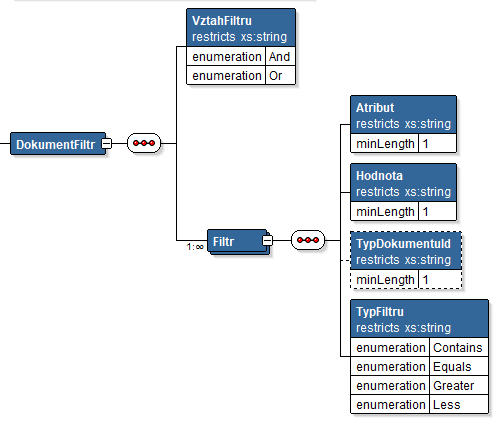
\includegraphics[width=0.6\linewidth]{./images/DokumentFiltr.png}} 
  \caption{Struktura filtru dokumentů.} 
\end{figure}

Struktura se používá během volání metody \kiinlinecode{text}{!}{ProfilSpisu}, kde slouží k~filtrování dokumentů ve spisu.
Důležitou roli hraje v~komunikaci s~IS/STAG, kdy jsou zakládány velké spisy přijímacích řízení. Pro každou fakultu existuje pro daný rok právě jeden spis přijímacích řízení a v~něm se nachází veškeré písemnosti (dokumenty) všech uchazečů dané fakulty. V~případě rozhodnutí o~přijetí je uchazeči založen spis studenta, do kterého se přetřídí všechny dokumenty, které se ho týkají. Identifikace uchazeče se provádí na základě jeho osobního čísla. Pomocí struktury \kiinlinecode{text}{!}{DokumentFiltr} obsažené v~žádosti o~profil spisu přijímacího řízení IS/STAG získá dokumenty konkrétního uchazeče a ty je schopen ze spisu vytřídit a zatřídit je do spisu studenta.


\subsection{Dynamické atributy (MAttr)}
\begin{figure}[h]
  \centerline{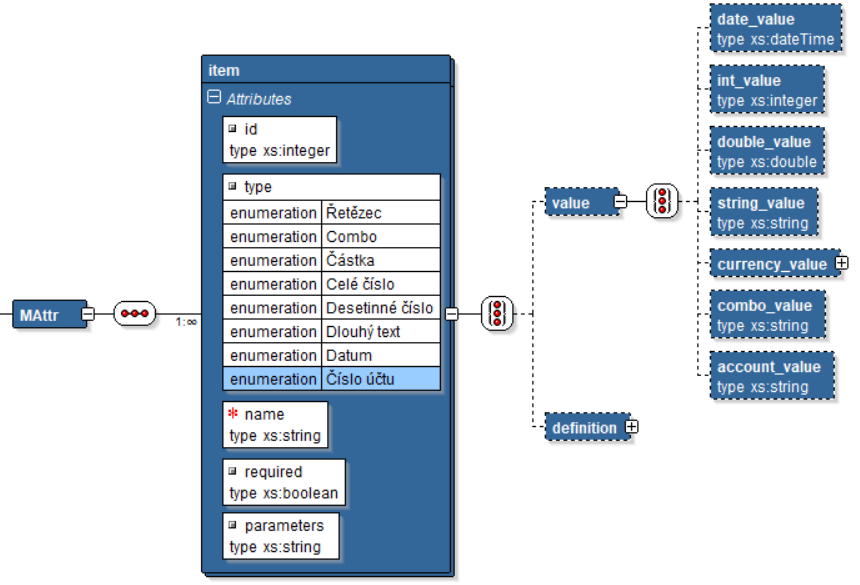
\includegraphics[width=0.6\linewidth]{./images/MAttr.png}} 
  \caption{Struktura dynamických atributů typu dokumentu.} 
\end{figure}

Struktura slouží k~přenosu dynamických atributů definovaných typem dokumentu. Pokud jde o~volání metody \kiinlinecode{text}{!}{ProfilDokumentu}, nese informace evidované u~konkrétního dokumentu. Pokud se jedná o~metodu \kiinlinecode{text}{!}{DokumentZalozeni}, tak nese inforamce o~dynamických atributech, které se mají danému dokumentu vytvořit.
V~případě vytváření dokumentu se kontroluje, jestli volání obsahuje všechny povinné atributy. V~opačném případě dokument nelze založit.

\subsection{UdelitZpristupneni}
\begin{figure}[h]
  \centerline{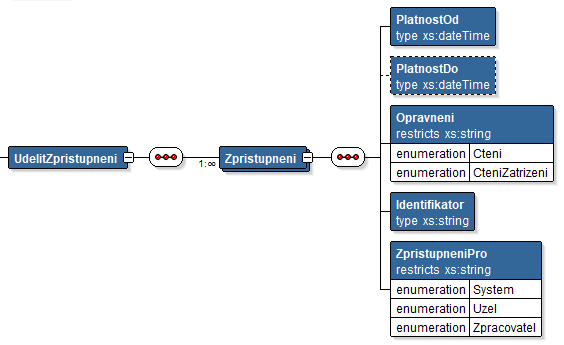
\includegraphics[width=0.6\linewidth]{./images/UdelitZpristupneni.png}} 
  \caption{Struktura zpřístupnění dané entity.} 
\end{figure}

Struktura upravující práva k~danému dokumentu nebo spisu. Více v~kapitole o~zpřístupnění.

\subsection{Další struktury}
\begin{figure}[h]
  \centerline{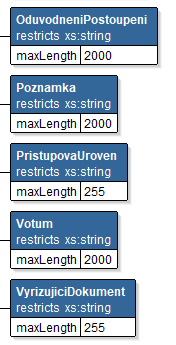
\includegraphics[width=0.2\linewidth]{./images/Ostatni.png}} 
  \caption{Další doplňující struktury.} 
\end{figure}
\begin{itemize}
	\item OduvodneniPostoupeni\\
	V~případě komunikace ISSD s~ERMS může nastat situace, kdy je dokument nebo spis postoupen do ISSD, ale ten zjistí, že daná entita pro něj nemá žádný význam. V~takovém případě entitu vrací do výhradní správy ERMS a může v~doplňujících datech připojit odůvodnění postoupení zpět do ERMS. Tento text se pak zobrazuje v~detailu dané entity jako poznámka.
	
	Příkladem může být vícenásobně zaevidovaná faktura. Během postoupení dokumentu do SAP se zjistí, že pro daného dodavatele je faktura již evidována, a tak ji SAP vrátí zpět do ERMS s~odůvodněním postoupení. Zpracovatel je pak prostřednictvím této poznámky informován, proč se daný dokument vrátil a může s~touto informací dále pracovat (například doručený dokument stornovat).
	\item Poznamka.\\
	Struktura obsahující poznámku evidovanou k~danému dokumentu nebo spisu.
	\item Varovani.\\
	 Pokud nastane přerušení komunikace a ISSD neobdrží potvrzení volání (například timeout během komunikace), dle best practices\cite{o01} volání opakuje. ERMS opakované volání přijme, během vykonávání volání se zjistí, že je daná entita již evidována, a proto odpověď doplní varováním, že se jedná o~opakované volání založení entity. V~takovém případě se profil entity do odpovědi poskládá z~dat, které eviduje ERMS a je zodpovědností ISSD, aby ověřil, že přijaté potvrzení obsahuje data, která posílal.
	 \item EvidencniCislo.\\
	 V~případě doručeného dokumentu může v~agendě ISSD sloužit jako identifikátor daného záznamu.
	 \item PristupovaUroven.\\
	 Standardní struktury nemají možnost přenášet informaci o~přístupové úrovni daného dokumentu.
	 \item Votum.\\
	 Krátký popis spisu.
	 \item VyrizujiciDokument.\\
	 Klíčová informace v~případě vyřízení dokumentu nebo spisu dokumentem standardní struktury neumožňují přenášení informace o~vyřizujícím dokumentu.
	 
Jedná se o~identifikátor vyřizujícího dokumentu. V~případě profilu spisu nebo dokumentu má informativní charakter. V~případě události vyřízení odkazuje na existující evidovaný dokument (který má daný ISSD ve výhradní správě).
	 \item AnalogovyDokument.\\
	 Používání webových služeb předpokládá manipulaci s~digitálními dokumenty. Tato struktura umožňuje během zakládání dokumentu určit, že se jedná o~evidenci analogového dokumentu, což má několik dopadů pro manipulaci s~daným dokumentem.
	 
Analogový dokument nelze vypravit digitální formou (e-mail, datová schránka) a nelze k~němu připojovat komponenty.
	 \item ErmsExportDokument a ErmsExportSpis.\\
	 Jedná se o~kontejnery přenosu dat buď z~jiné agendy do ERMS a nebo z~ERMS do jiné agendy. Struktury byly využity pro migraci historických dat předchozí agendy MAGION.
\end{itemize}


\newpage
\section{Zpřístupnění entit}
\begin{figure}[h]
  \centerline{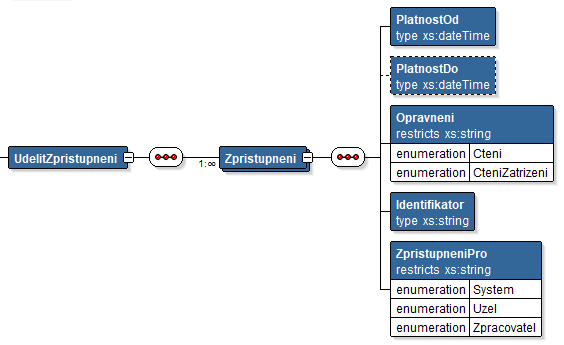
\includegraphics[width=0.9\linewidth]{./images/UdelitZpristupneni.png}} 
  \caption{Struktura zpřístupnění.} 
\end{figure}
Struktury \kiinlinecode{text}{!}{UdelitZpristupneni} a \kiinlinecode{text}{!}{OdebratZpristupneni} definované v~namespace erms-ext slouží pro řízení přístupu k~entitám. Nastavení zpřístupnění je možné provádět pouze nad entitami, které jsou aktuálně ve výhradní správě daného ISSD (systém, který volá dané metody). Zpřístupnění lze časově omezit.

Struktura \kiinlinecode{text}{!}{UdelitZpristupneni} obsahuje seznam jednotlivých zpřístupnění, která se mají nastavit. V~případě, že během vykonávání dojde k~chybě (například daná entita podle identifikátoru není nalezena, a proto ji nelze udělit zpřístupnění), dochází k~rollback celého volání. Transakce je tedy na úrovni celého volání, nikoliv na úrovni jednotlivých položek seznamu.

Atribut \kiinlinecode{text}{!}{Opravneni} slouží v~případě udělení zpřístupnění pro spis k~určení, jestli má daný subjekt oprávnění pouze daný spis číst a nebo jestli je mu umožněno do něj zatřiďovat nové dokumenty. Pro ostatní entity, které nejsou spisy, se uvažuje pouze hodnota \kiinlinecode{text}{!}{Cteni}.

Atribut \kiinlinecode{text}{!}{ZpristupneniPro} určuje, jakému typu subjektu se zpřístupnění uděluje. \kiinlinecode{text}{!}{Zpracovatel} je identifikován pomocí identifikátoru uživatele, \kiinlinecode{text}{!}{Uzel} pomocí kódu organizační jednotky a \kiinlinecode{text}{!}{System} pomocí kódu systému, který byl registrován pro komunikaci skrze webové služby.

Pokud má daná entita (spis/dokument/komponenta) nastavené zpřístupnění pro systém, na straně systému ERMS se neověřuje, jestli je žadatel o~čtení přiřazeným zpracovatelem dané entity. Pouze se zaloguje pokus o~přístup tohoto žadatele (buď success a nebo fail).

\subsection{Zpřístupnění pomocí dědičnosti}
Zpřístupnění dané entity znamená, že jsou zpřístupněny i podřízené entity. U~dokumentu jsou zpřístupněny i komponenty připojené k~tomuto dokumentu. U~spisu jsou zpřístupněny všechny vložené dokumenty (a jejich komponenty). Pokud dojde k~vytřídění dokumentu ze spisu, dochází k~automatickému zrušení zpřístupnění vytříděného dokumentu (a jeho komponent).

V~případě zatřídění dokumentu do spisu, který měl nastavené zpřístupnění, je toto nastavení převzato.

\subsection{Explicitní zpřístupnění}
Kromě zpřístupnění pomocí dědičnosti lze explicitně určit, které entity mají být zpřístupněny (například vybraný dokument ze spisu je zpřístupněn, ale celý spis ne). V~takovém případě je explicitní zpřístupnění zachováno i pokud dojde k~vytřídění ze spisu (který zpřístupnění nastavené neměl). Zpřístupnění se nastaví i pro podřízené entity.

\subsection{Krajní případ}
Nastavení zpřístupnění je možné provádět i pomocí webového rozhraní.
Ukázkový příklad:
\begin{enumerate}
	\item Z~ERMS je do ISSD postoupen dokument.
	\item ISSD založí spis a do něj daný dokument zatřídí.
	\item ISSD nastaví zpřístupnění spisu pro sebe a vrátí spis zpět do ERMS.
	\item Spis není uzavřen, takže zpracovatel může se spisem v~ERMS pracovat.
	\item Zpracovatel zruší zpřístupnění pro ISSD.
	\item ISSD ztratí přístup.
	\item Toto je korektní chování systému.
\end{enumerate}

\subsection{Odebrání zpřístupnění pomocí dědičnosti}
Pokud dojde k~odebrání zpřístupnění dané entity, odeberou se i zpřístupnění podřízených entit (kromě explicitně nastavených zpřístupnění, která zůstávají).

\subsection{Změna výhradní správy}
Změna výhradní správy entity (např. spis je postoupen zpět do ERMS) neovlivní nastavená zpřístupnění. Nadále zůstávají práva ke čtení (profilSpisuZadost, profilDokuemntuZadost, souborZadost). Po skartačním řízení dané entity přístup zůstane, ale struktura již neobsahuje obsah komponent a metaatributy.

\newpage
\section{Napojení systémů IS/STAG, SAP, CES a kofax (skenovací linka)}
Integrace informačních systémů, které jsou na UP provozovány, je aplikací popisovaných principů komunikace mezi ISSD a ERMS.

\subsection{CES}
\newacronym{CES}{CES}{Centrální evidence smluv}
\gls{CES} slouží k~evidenci všech uzavřených smluv na UP, k~vyhledávání konkrétní smlouvy podle různých kritérií a k~získání celkového přehledu smluv pro oprávněné uživatele.

\begin{figure}[h]
  \centerline{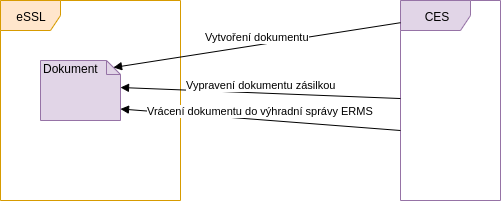
\includegraphics[width=0.9\linewidth]{./images/CESworkflow.png}} 
  \caption{Workflow systému CES.} 
\end{figure}

Systém CES je napojen na ERMS prostřednictvím webových služeb a plní roli ISSD. To znamená, že má registrovaný endpoint pro zpětné notifikace.
Workflow systému CES začíná vytvořením dokumentu. Následně se vytváří odchozí zásilka a prostřednictvím datové schránky se zásilka vypravuje do registru smluv.

Pro zjištění výsledku zveřejnění v~registru smluv CES implementuje vlastní rozhraní a tato komunikace neprobíhá skrze ERMS.


\subsection{SAP}

\newacronym{SAP}{SAP}{Podnikový a manažerský informační systém v~oblasti plánování podnikových zdrojů (ERP)}

\gls{SAP} plní roli ISSD včetně asynchronní komunikace.

\begin{figure}[h]
  \centerline{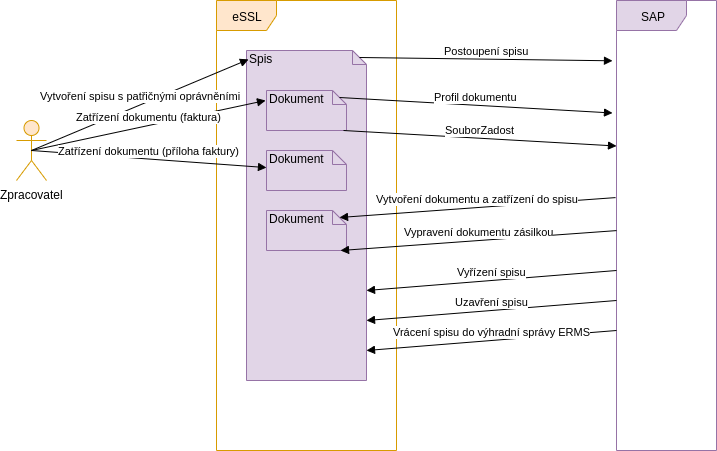
\includegraphics[width=0.9\linewidth]{./images/SAPworkflow.png}} 
  \caption{Workflow systému SAP.} 
\end{figure}


Workflow začíná na straně ERMS, kde zpracovatel vytvoří spis a nastaví mu patřičná zpřístupnění. Zejmnéna možnost systému ERMS zatřizovat dokumenty do spisu.

V~ERMS existuje systém zpřístupnění spisů pro zpracovatele a spisové uzly, bez kterých nemá možnost nikdo jiný než přiřazený zpracovatel se spisem manipulovat. Tento princip se dodržuje i v~případě, kdy je spis ve výhradní správě ISSD. Pokud má spis nastavené zpřístupnění pouze pro systém ERMS, může do něj zatřizovat pouze přiřazený zpracovatel. Toto zpřístupnění je vnímáno tak, že přiřazený zpracovatel pracuje s~více agendami najednou a pro zvýšení pohodlnosti pak může s~danou entitou manipulovat v~obou agendach bez potřeby předávání výhradní správy mezi agendami. Pokud je chtěné, aby do spisu mohl dokumenty zatřizovat i další zpracovatel, aplikují se pravidla zpřístupnění pro zpracovatele a spisové uzly i v~případě výhradní správy mimo ERMS. Oprávnění se týká pouze zatřizování nových dokumentů do spisu. V~případě potřeby vytřídění dokumentu ze spisu nebo další manipulace se spisem platí výhradní správa daného ISSD a modifikace prostřednictvím dalších agend není přípustná.

Pro zachování konzistence dotčených entit se v~případě zatřízení nového dokumentu do spisu určuje zpracovatelem dokumentu zpracovatel spisu. Dále dochází k~převzetí výhradní správy dokumentu tak, aby korespondovala s~výhradní správou spisu.

Životní cyklus spisu na straně SAP končí vyřízením a uzavřením spisu. Následně je potřeba spis vrátit do výhradní správy ERMS, kde ho poslední určený zpracovatel může předat na spisovnu.
Pokud spis bude mít nastavené zpřístupnění systému SAP, bude umožněno čtení dat (získání profilu spisu) i po vrácení výhradní správy ERMS.
 

\subsection{IS/STAG}
IS/STAG je informační systém studijní agendy vysoké školy, univerzity nebo vyšší odborné školy. Jedná se o~celouniverzitní systém určený pro administraci studia, který eviduje kreditní i nekreditní systém studia.

\begin{figure}[h]
  \centerline{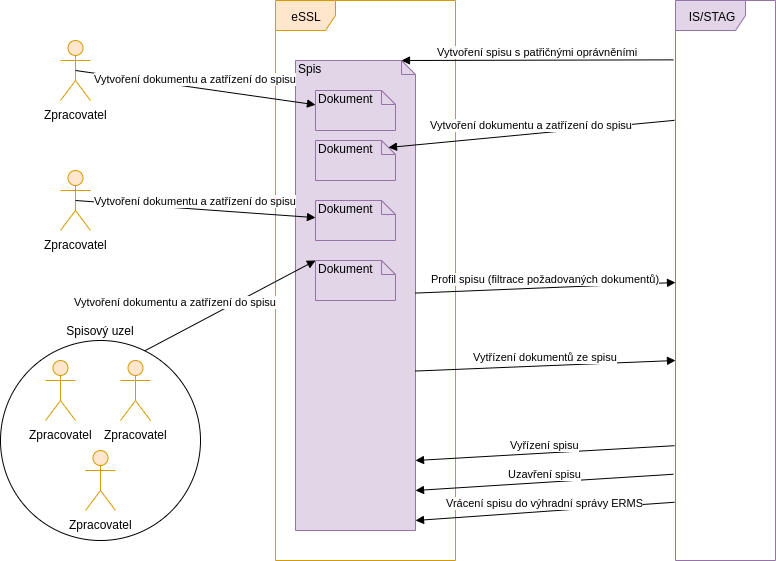
\includegraphics[width=0.9\linewidth]{./images/STAGworkflow.png}} 
  \caption{Workflow systému IS/STAG.} 
\end{figure}
V~případě systému IS/STAG se jedná o~jednostrannou komunikaci (směr z~IS/STAG do ERMS) a není tak plnohodnotným ISSD (pouze se pro komunikaci používá stejné synchronní rozhraní).

Workflow začíná na straně ISSD. Systém založí spis, který obsahuje v~doplňujících datech všechna potřebná zpřístupnění. Existují dva typy spisů. Prvním typem je spis elektronických přihlášek, druhým typem jsou spisy studentů.

Do spisů elektronických přihlášek se zatřizují nové dokumenty prostřednictvím IS/STAG i prostřednictvím ERMS díky nastaveným zpřístupněním. Po přijetí uchazeče ke studiu se vytřizují jeho dokumenty ze spisu přihlášek a zatřizují se do spisu studenta. Pro tento krok se využívá filtrace dokumentů. Základní použití filtru spočívá ve filtrování napříč všemi typy dokumentů a vyhledávají se všechny dokumenty, které obsahují vyhledávané osobní číslo (jednoznačný identifikátor studenta). V~průběhu studia mohou vznikat další dokumenty, které se do spisu studenta zatřizují. I~v~tomto případě platí zachování konzistence dotčených entit jako u~SAP (dokumenty přebírají určeného zpracovatele spisu a přebírá se výhradní správa shodná s~výhradní správou spisu).

Životní cyklus spisu na straně IS/STAG končí vyřízením a uzavřením spisu. Následně je potřeba spis postoupit do výhradní správy ERMS, kde ho poslední určený zpracovatel může předat na spisovnu.
 
Filtrace dokumentů může být dvojího typu:
\begin{enumerate}
	\item Filtruje se dle předem definované množiny atributů dokumentu:
	\begin{itemize}
		\item Id.
		\item Vec.
		\item CisloJednaci.
		\item PuvodniCisloJednaci.
		\item DatumVytvoreni.
		\item VytvorilKdo (identifikátor uživatele).
		\item SerioveCislo.
		\item VecnaSkupinaId.
		\item SpisovaZnacka.
		\item Zpracovatel (identifikátor uživatele).
		\item TypDokumentuId.
		\item Barcode (čárový kód).
		\item Vlastnik (kód org. jednotky).
		\item Komentar.
		\item Vyrizen (hodnota ano/ne).
	\end{itemize}
	\item Filtrace v~dynamickych atributech daneho typu dokumentu.\\
	Atribut \kiinlinecode{text}{!}{TypDokumentuId} se vyplní v případě, že se má filtrovat na základě vybraného typu dokumentu. Pokud se daný atribut nevyplní, dohledává se daná fráze ve všech dynamických atributech, které se můžou u~všech typů dokumentů vyskytovat.
\end{enumerate}  

Filtr atributů lze kombinovat a spojovat logickými spojkami and a or (všechny přítomné filtry budou spojeny stejnou logickou spojkou).

\subsection{Skenovací linka}
Skenovací linka pracuje se soubory formátu PDF. Jedná se o~desktopovou aplikaci, která načítá binární obsah těchto souborů a nahrává je do ERMS za účelem spárování s~dokumentem.

Pro práci s~aplikací je vyžadováno přihlášení.
\begin{figure}[h]
  \centerline{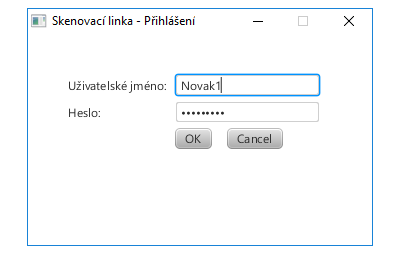
\includegraphics[width=0.5\linewidth]{./images/ScanLinePrihlaseni.png}} 
  \caption{Přihlašovací obrazovka skenovací linky.} 
\end{figure}

Po přihlášení uživatel vidí v~horním řádku Počet souborů k~odeslání (počet souborů nacházejících se ve zdrojové složce), které se po stisku lačítka Načíst připraví ke zpracování.

V~následujícím kroku má uživatel na výběr z~několika možností:
\begin{enumerate}
	\item Tlačítko Hromadně odešle všechny soubory ze zdrojové složky do ERMS.
	\item Tlačítko Odeslat odešle pouze aktuálně zobrazený soubor.
	\item Tlačítko Vynechat aktuálně zobrazený soubor přeskočí a zobrazí následující soubor.
	\item Tlačítko Smazat aktuálně zobrazený soubor odstraní ze zdrojové složky a zobrazí následující soubor.
\end{enumerate}

Ve spodní stavové liště je uživatel informován o~výsledku operace.

Pro konfiguraci skenovací linky slouží soubor config.properties s~následujícími atributy definovanými v~tabulce \ref{tab:ScanLineConfig}.
\begin{table}
\begin{center}
\caption{Konfigurační parametry skenovací linky}\label{tab:ScanLineConfig}
\scalebox{0.95}{\begin{tabular}{>{\bfseries}l L{8cm}}
{\normalfont Atribut} & {\normalfont Popis} \\
\hline

source	&	Zdrojová složka s~PDF soubory. \\
destination	&	Cílová složka, kam se ukládají zpracované soubory. \\
url	&	Adresa serveru včetně portu pro připojení skrze remote interface. \\
username	&	Přihlašovací jméno autorizace skenovací linky. \\
passwd	&	Heslo autorizace skenovací linky. \\
mailRoomID	&	Kód podatelny, kam se má sken nahrát. \\

\end{tabular}}
\end{center}
\end{table}

Externí skenovací linka se autorizuje stejným principem jako ISSD.\footnote{Existuje pro ni registrace ISSD popsaná v~kapitole \ref{ch:issd}.} Dále však nevyužívá rozhraní webových služeb, ale Java RMI.\footnote{\url{https://docs.oracle.com/javase/8/docs/platform/rmi/spec/rmi-objmodel5.html}} Použití remote interface je možné z~toho důvodu, že skenovací linka je Java aplikace a ERMS běží na aplikačním serveru jBoss.

\newpage
\begin{figure}[h]
  \centerline{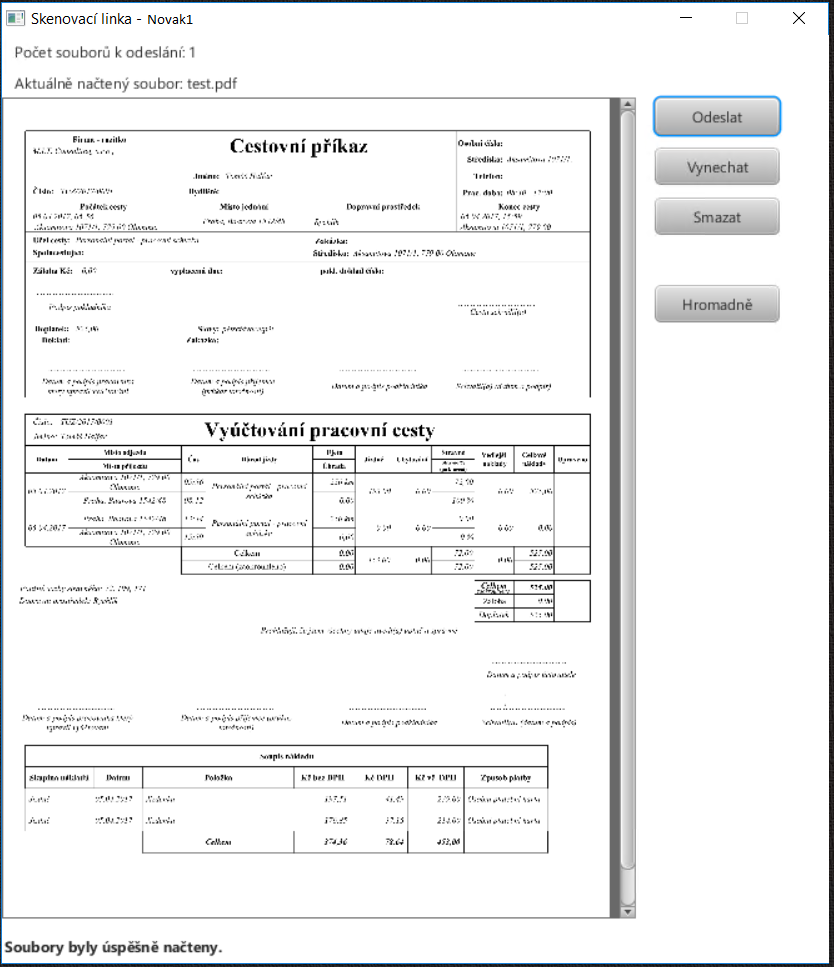
\includegraphics[width=1\linewidth]{./images/ScanLine2.png}} 
  \caption{Prostředí skenovací linky.} 
\end{figure}

\newpage
\section{Logování}
\begin{figure}[h]
  \centerline{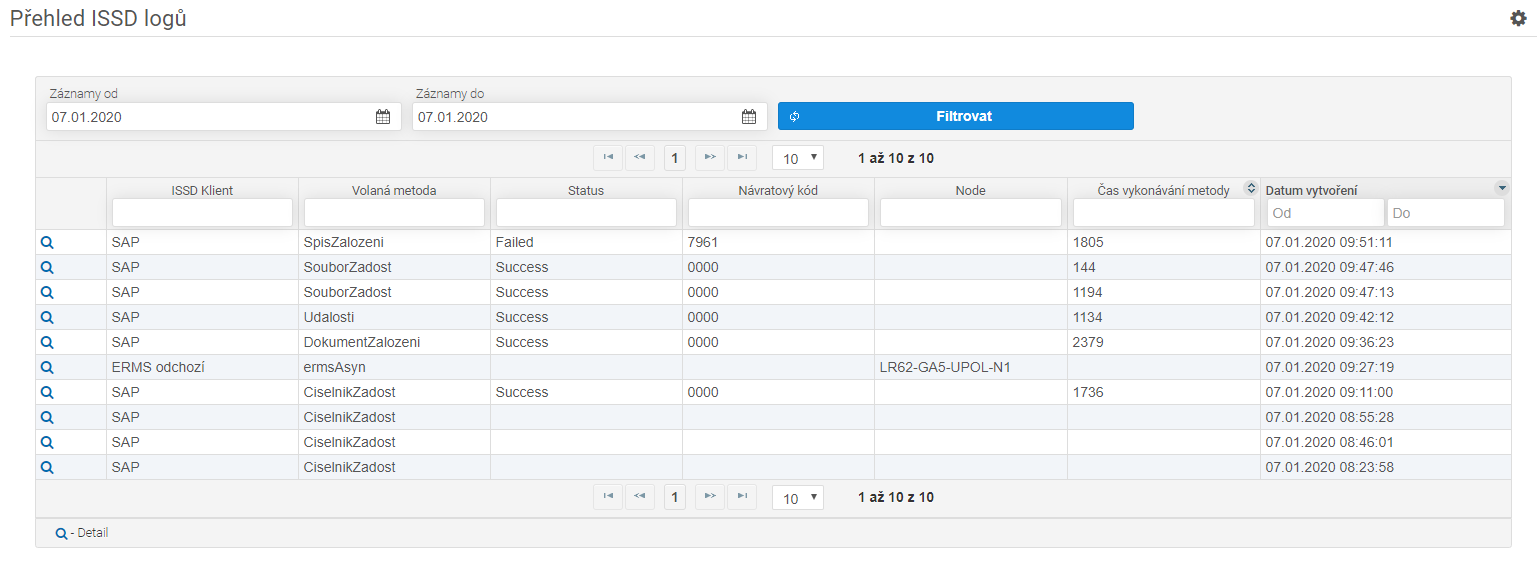
\includegraphics[width=0.9\linewidth]{./images/LogovaniWeb.png}} 
  \caption{Přehled logovaných volání.} 
\end{figure}
Logování je způsob, jak může administrátor systému zjistit, že je probíhající komunikace ERMS s~ISSD v~pořádku. Dochází k~logování každého volání webových služeb. V~přehledové tabulce uživatel vidí záznamy příchozí i odchozí komunikaci. Z~důvodu velkého množství jednotlivých událostí lze pro přehlednost záznamy v~tabulce filtrovat dle času.
\begin{figure}[h]
  \centerline{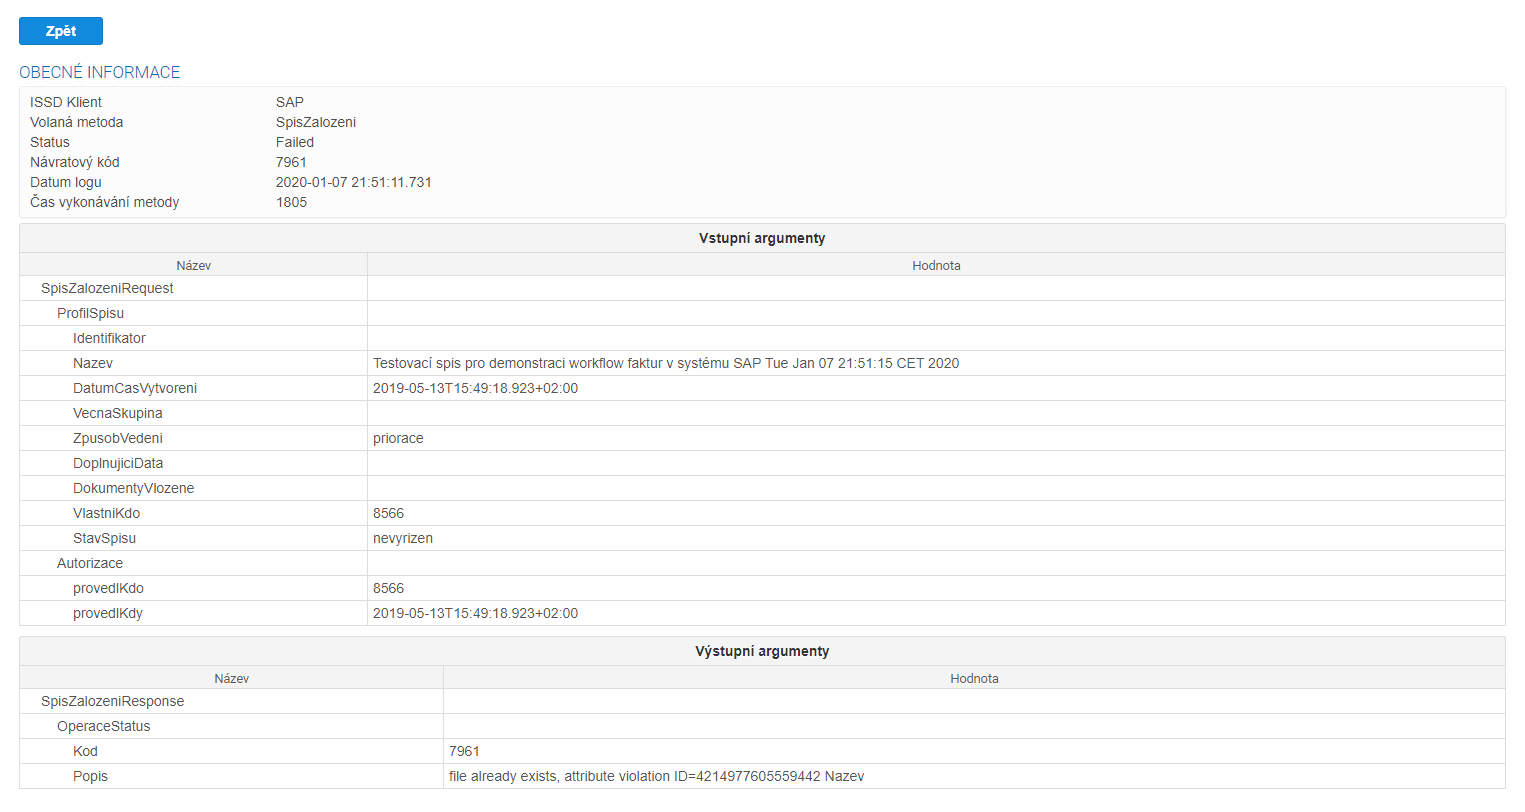
\includegraphics[width=0.9\linewidth]{./images/LogovaniWebDetail.png}} 
  \caption{Detail volání.} 
\end{figure}
U~každého volání lze zobrazit detail, kde se přehledně ukazuje struktura volání a její vstupní a výstupní argumenty.

\newpage
\section{Testování}
Pro účely testování funkčnosti rozhraní bylo použito softwaru SOAP UI. Projekt je uložen jako XML soubor, který obsahuje připravená data pro volání jednotlivých webových metod. Dále obsahuje ucelené testovací scénáře, které se skládají z~více kroků.

\subsection{Testovací scénáře pro jednotlivé informační systémy}
Pro každý informační systém, který je s~ERMS integrován, vznikl testovací scénář, který popisuje jeho workflow.
\begin{enumerate}
	\item Testovací scénář pro IS/STAG:
	\begin{itemize}
		\item Založení spisu přijímacího řízení se zpřístupněním.
		\item Vložení několika dokumentů do spisu (různé typy dokumentů).
		\item Získání profilu spisu s~aplikovaným filtrem dokumentů podle oborového čísla.
		\item Založení spisu studenta.
		\item Přetřízení získaných filtrovaných dokumentů ze spisu přijímacího řízení do spisu studenta.
		\item Získání profilu spisu studenta pro potvrzení přítomnosti přetřízených dokumentů.
		\item Předání spisu do výhradní správy ERMS (vyřízení, uzavření, vrácení).\footnote{Simulace uzavření spisu přijímacího řízení pro daný akademický rok. Následně se vytváří nový spis pro následující akademický rok.}
		\item Předání spisu studenta  do výhradní správy ERMS (vyřízení, uzavření, vrácení).\footnote{Simulace ukončení studia.}
	\end{itemize}
	\item Testovací scénář pro SAP: \\
	Následující body slouží k~simulaci workflow, které zpracovatel provádí na straně ERMS dříve, než dojde k~předání výhradní správy systému SAP.
	\begin{itemize}
		\item Založení spisu se zpřístupněním.
		\item Založení dokumentu do spisu (typ faktura).
		\item Založení komponenty a její připojení k~dokumentu (simulace přijetí faktury například e-mailem).
	\end{itemize}		
	Dalším krokem by bylo postoupení spisu do výhradní správy SAP. Protože se předchozí body provedly pomocí volání webových služeb, jsou dotčené entity již ve správě SAP.
	\begin{itemize}
		\item Čtení obsahu komponenty daného dokumentu.
		\item Vytvoření dokumentu a zatřízení do spisu.
		\item Vytvoření komponenty a připojení k~dokumentu.
		\item Vypravení zásilky.
		\item Předání spisu do výhradní správy ERMS (vyřízení, uzavření, vrácení).
	\end{itemize}
	\item Testovací scénář pro CES:
	\begin{itemize}
		\item Vytvoření dokumentu.
		\item Připojení komponenty.
		\item Vypravení dokumentu e-mailem nebo datovou schránkou.
		\item Vrácení dokumentu do výhradní správy ERMS.
	\end{itemize}
\end{enumerate}

\subsection{Spuštění testovacích scénářů pomocí SOAP UI}
\begin{figure}[h]
  \centerline{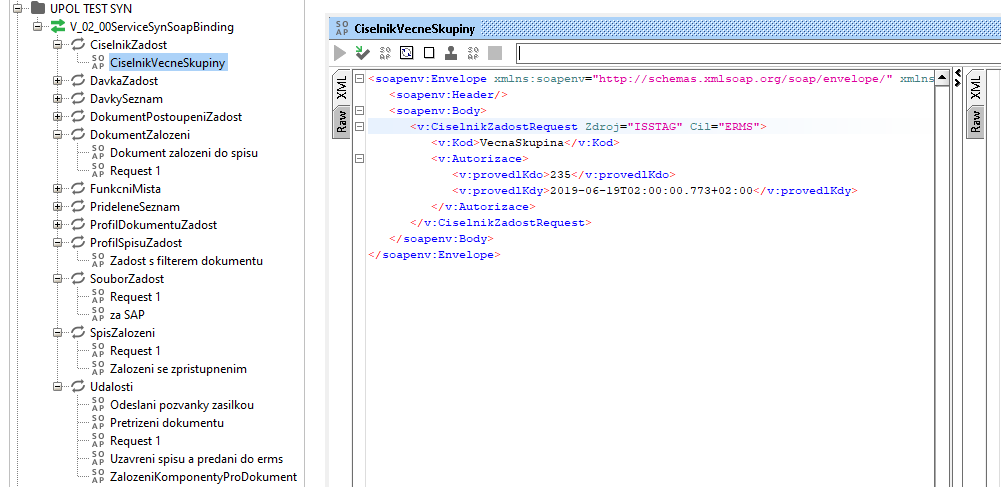
\includegraphics[width=0.9\linewidth]{./images/SOAPUI2.png}} 
  \caption{Připravená volání metod v~SOAP UI.} 
\end{figure}
\begin{enumerate}
	\item Import projektového souboru.
	\item Přehled připravených událostí k~volání.
	\item Spuštění testovacího scénáře.
\end{enumerate}

Před spuštěním testovacího scénáře, který je složený z~jednotlivých kroků, dochází ke generování potřebných identifikátorů.\footnote{Testovací scénář simuluje fungovaní ISSD a dle definice je správa identifikátorů v~roli ISSD.} Tento krok je potřebný k~tomu, aby se testovací scénář mohl spouštět opakovaně. Po dokončení volání je možné zobrazit výsledky pro jednotlivé metody. Ve všech případech by měla být odpověď ERMS návratový kód \kiinlinecode{text}{!}{0000}, který znamená úspěšné zpracování požadavku.

\newpage
\begin{figure}[h]
  \centerline{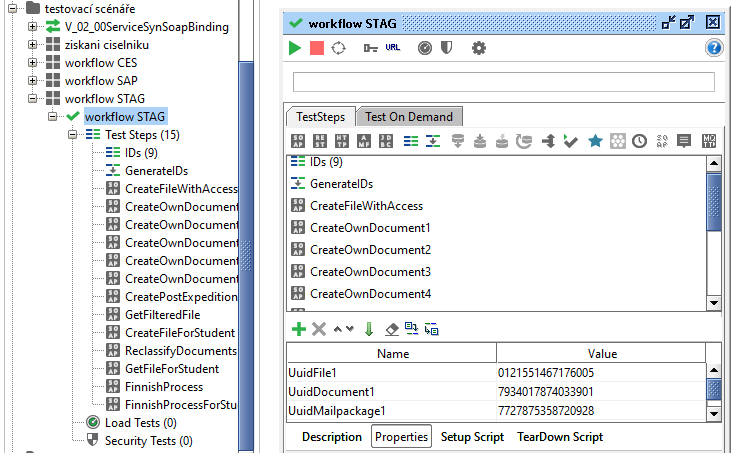
\includegraphics[width=0.9\linewidth]{./images/TestSuite.png}} 
  \caption{Testovací scénář pro demonstraci workflow IS/STAG.} 
\end{figure}

\newpage
\section{Diskuze -- možná rozšíření}
Z~praktického používání asynchronní komunikace vyvstala potřeba notifikovat administrátora o~problémech přerušení asynchronní komunikace.

Analýzou důvodů přerušení komunikace vzniklo několik bodů, které je možné kontrolovat a v~případě neočekávaného chování zasílat e-mailové notifikace o~vzniklém problému:
\begin{enumerate}
	\item Počet opakování aktuálně odesílané dávky překročí určitou mez.\\
	K~pokusu o~odeslání dávky dochází každých 17 sekund. Navrhovaná mez je 5 až 10 opakování.
	\item Počet vytvořených událostí, které se nezařadily do žádné dávky, překročí určitý počet.\\
	Příčinou takového stavu může být v~případě postupování dokumentu nebo spisu stav, kdy systém čeká na dokončení transformace komponenty. Jelikož je tento proces také asynchronní a v~některých případech dochází k~zablokování transformační fronty, může na transformaci čekat velké množství komponent. Limit pro počet událostí se pohybuje v~rozmezí 20 až 50. Víc čekajících entit k~postoupení může značit přehlcení systému, a v~takovem případě je chtěná pozornost administrátora.
		
	Z~důvodu udržení rozumné velikosti zprávy zasílané přes SOAP je nastavený limit počtu událostí v~jedné dávce na 100. Pokud došlo k~zastavení sestavování událostí do odchozí dávky a k~následnému opětovnému spuštění, stalo se, že se všechny čekající události shlukly do jednoho volání. Tento limit zajistí rovnoměrnější rozložení událostí a předchází případnému zahlcení ISSD.
	\item Zohlednění počtu iterací, ve kterých se přeskočilo zařazení dané události do dávky kvůli čekající transformaci.	
	\item Počet odeslaných dávek ve stavu \kiinlinecode{text}{!}{SENT} překročí hranici 20 až 50.\\
	Velké množství nepotvrzených dávek může značit problém se zpracováním na straně ISSD. Systém nové dávky přijímá (splňují všechny formální body pro přijetí dávky), ale nedochází k~jejich zpracování. V~takovém případě je opět žádoucí pozornost administrátora.
	\item Odchozí dávka je ve stavu \kiinlinecode{text}{!}{SENT} po delší dobu (například 30 minut).\\
	Jedná se o~stejný případ jako v~předchozím bodě. Na straně ISSD nedošlo k~odeslání potvrzující zprávy, že dávka byla zpracována. V~tomto případě je potřeba zohlednit interval, ve kterém ISSD zpracovává příchozí dávky.
\end{enumerate}

Identifikovat problémy v~komunikaci lze i v~případě synchronního rozhraní. V~logovací tabulce volání synchronního rozhraní se objeví stav \kiinlinecode{text}{!}{Fail}. Jedná se o~situaci, kdy ISSD volá synchronní rozhraní a během vykonávání se jako odpověď vrací chybový kód. V~testovacím prostředí to může být běžný jev, když se snaží ISSD integrovat, ale v~provozním prostředí to může znamenat neočekávaná data v~některé struktuře. Pro analýzu chybových volání se ukládají vstupní i výstupní argumenty volání.

%%administratorska moznost odseknuti davek. prazdna ermsAsyn.
%%funguje v aktualnim pripade, kdy z erms odchazi postoupeni a notifikace o vypraveni, informace o skartacich  popsat problematiku kodovani v SAP, ze nebyl schopny prijmout a volani koncilo na SOAP Exception
V případě aplikace systému zpřístupnění dochází k nejasnostem týkajících se výhradní správy nad daným dokumentem nebo spisem. Jedná se o nadstandardní chování za účelem zjednodušení práce a omezení kroků potřebných k dosažení cíle, které je specifické pro konkrétní implementaci ERMS. Uvažujme následující situaci: V ERMS vznikne spis, do kterého chce ISSD zatřídit nový dokument. V takovém případě se spis musí předat do výhradní správy daného ISSD, aby tuto operaci mohl vykonat. Následně ale potřebuje zpracovatel do spisu zatřídit dokument, který zaevidoval v ERMS. Musí dojít ke změně výhradní správy z ISSD do ERMS, aby tento krok bylo možné vykonat.

Takový pracovní postup je typický pro systém IS/STAG i pro SAP. Spis je držen ve výhradní správě ISSD a zpracovatel zaeviduje v ERMS dokument (v případě IS/STAG se může jednat o žádost studenta, v případě SAP o fakturu). Aplikací principů zpřístupnění odpadá nutnost změnit výhradní správu spisu (z ISSD do ERMS) za účelem zatřízení dokumentu a následně opětovně vrátit spis do ISSD. Pro zachování konzistence se považují dokumenty ve spisu ve stejné výhradní správě, v jaké je držený spis. Pokud by se tak nedělo, prakticky by se znemožnila veškerá práce se spisem nebo s dokumenty. Odpovědí volání webových metod by byl chybový návratový kódu, že operaci nelze provést, protože daná entita není ve výhradní správě daného ISSD.





%% Závěry práce. V jazyce práce a anglicky. Text pro jiný než
%% nastavený jazyk práce (nepovinným parametrem language makra
%% \documentclass, výchozí český) se zadává použitím makra s uvedením
%% jazyka jako nepovinného parametru.
\begin{kiconclusions}
Diplomová práce měla za cíl seznámení s~doménou problematiky spisové služby, která plní v~organizaci roli hlavního komunikačního kanálu. Existuje několik odborných agendových specializovaných systémů, pro které je výhodné a žádoucí být integrován se spisovou službou. 

Práce popsala základní principy komunikace definované národním standardem včetně analýzy nedostatků s~návrhem a implementací doplňujících struktur tak, aby struktury byly co nejobecnější a aby bylo pro uživatele možné používat všechny komunikující informační sysytémy pohodlně a efektivně. 

Aplikace metodiky synchronní a asynchronní komunikace definované národním standardem společně s~navrženými rozšiřujícími strukturami byla využita pro integraci agendových informačních systémů CES, IS/STAG a SAP, které jsou na UP provozovány. V případě CES a SAP se jedná o plnohodnotné ISSD z pohledu standardu, protože implementují rozhraní pro notifikace směrem z ERMS. Systém IS/STAG komunikuje pouze směrem k ERMS, neimplementuje rozhraní pro notifikace a tak není považován za ISSD. Využívá ale stejné synchronní rozhraní.

V případě systémů SAP a IS/STAG bylo využito i principů zpřístupnění za účelem pohodlnější a efektivnější práce. Tento systém zpřístupnění není pokrytý národním standardem.

Text diplomové práce obsahuje příklady komunikace mezi systémy, aby mohl sloužit jako technický manuál v~případě nutnosti integrace dalších agendových systémů.

Nedostatky aktuální verze národního standardu analyzované v práci, byly předány jako podněty pracovní skupině NSESSS, \footnote{\url{http://www.cnz.cz/odborne-aktivity/pracovni-skupina-nsesss/}} která se zabývá aktualizací standardu a vydáváním nových verzí.
\end{kiconclusions}

\begin{kiconclusions}[english]
The aim of the diploma project was to introduce the domain of the Electronic
Record Management System, which fulfills the role of the main communication channel
in the organization. Several professional and specialized systems for agenda exists which 
benefit from the integration with ERMS.

The thesis described the basic principles of communication defined by the national standard including the analysis of its shortcommings with a proposal and implementation of complementary structures in such a way for the structures to remain as general as possible and for making it possible for their users to efficiently and comfortably use every available communicating information system.

The application of synchronous and asynchronous communication defined by the national standard together with the proposed complementary structures were used for the integration of agenda information systems which are being operated by the Palacký University, specifically CES, IS/STAG and SAP. CES and SAP are considered full-fledged ISSD as defined by the national standard since they feature the implementation of notification interface with outbound communication from ERMS. The IS/STAG system only communicates towards ERMS, it does not implement the notification interface and is therefore not considered to be an ISSD. Nevertheless, it uses the same synchronous interface.

In the case of SAP and IS/STAG, principles of accessibility were used for the purpose of making the user experience more comfortable and efficient. The accessibility system is not covered by the national standard.

The text of the diploma project includes examples of communication between systems to serve as an instruction manual in the case of the necessity of integrating additional agenda systems.
\end{kiconclusions}

%% Přílohy obsahu textu práce, za makrem \appendix.
\appendix

%% Obsah přiloženého CD/DVD. Poslední příloha. Upravte podle vlastní
%% práce!
\section{Obsah přiloženého CD/DVD} \label{sec:ObsahCD}

\begin{description}

\item[\texttt{doc/}] \hfill \\
  Text práce ve formátu PDF, vytvořený s~použitím závazného stylu KI
  PřF UP v~Olomouci pro závěrečné práce, včetně všech příloh,
  a~všechny soubory potřebné pro bezproblémové vygenerování PDF
  dokumentu textu (v~ZIP archivu), tj.~zdrojový text textu, vložené
  obrázky, apod.

\item[\texttt{readme.txt}] \hfill \\
  Instrukce pro instalaci a~spuštění programu, včetně
  všech požadavků pro jeho bezproblémový provoz. / Webová adresa, na
  které je aplikace nasazena pro účel testování při tvorbě posudků
  práce a~pro účel obhajoby práce.

\end{description}

Navíc CD/DVD obsahuje:

\begin{description}

\item[\texttt{data/}] \hfill \\
  Ukázková a~testovací data použitá v~práci a~pro potřeby testování
  práce při tvorbě posudků a~obhajoby práce.

\item[\texttt{install/}] \hfill \\
  Instalátory aplikací, runtime knihoven a~jiných souborů potřebných
  pro provoz programu \textsc{Program} / webové aplikace
  \textsc{Webovka}, které nejsou standardní součástí operačního
  systému určeného pro běh programu / provoz webové aplikace.

\item[\texttt{literature/}] \hfill \\
  Vybrané položky bibliografie, příp.~jiná užitečná literatura
  vztahující se k~práci.

\end{description}

\newpage
\section{Ukázková volání}\label{sec:XMLVolani}
Následující část obsahuje příklady XML zpráv. Tato ukázková volání slouží pro snadnější orientaci programátora, který by potřeboval integrovat další ISSD. Výhoda ukázkových volání spočívá v přehlednosti nutných atributů k úspěšnému volání. Programátor tak nemusí v první fázi integrace provádět testování ve stylu blackbox a podle chybových návratových kódů zkoušet, které atributy jsou nutné pro úspěšné volání a které nikoliv. Příloha obsahuje pouze nejzbytnější ukázky použité v textu práce pro založení spisů, dokumentů a vypravení.

\begin{kicode}{XML}{kod:XML}{Založení vlastního dokumentu.}
<DokumentZalozeniRequest xmlns="http://nsess.public.cz/erms/v_02_00" 
    xmlns:ns2="http://mit-consulting.cz/erms-ext" Zdroj="CES" Cil="ERMS">
    <ProfilDokumentu>
        <Identifikator>
            <HodnotaID>9091015973527768</HodnotaID>
            <ZdrojID>CES</ZdrojID>
        </Identifikator>
        <Nazev>Testovací darovací smlouva Thu Jan 09 21:11:00 CET 2020</Nazev>
        <VecnaSkupina>
            <Identifikator>
                <HodnotaID>c0860f16-4fd3-4c1b-b6ce-c594f3d89420</HodnotaID>
                <ZdrojID>ERMS</ZdrojID>
            </Identifikator>
        </VecnaSkupina>
        <Poznamka>Testovací darovací smlouva</Poznamka>
        <PocetListu>0</PocetListu>
        <PocetPriloh>0</PocetPriloh>
        <DruhPriloh></DruhPriloh>
        <PocetListuPriloh>0</PocetListuPriloh>
        <DoplnujiciData>
            <ns2:Poznamka>Poznamka</ns2:Poznamka>
            <ns2:Poznamka>Testovací darovací smlouva</ns2:Poznamka>
        </DoplnujiciData>
        <VlastniKdo>8451</VlastniKdo>
        <StavDokumentu>nevyrizen</StavDokumentu>
    </ProfilDokumentu>
    <Autorizace>
        <provedlKdo>8451</provedlKdo>
        <provedlKdy>2019-05-13T15:49:18.923+02:00</provedlKdy>
    </Autorizace>
</DokumentZalozeniRequest>
\end{kicode}

\begin{kicode}{XML}{kod:XML}{Založení doručeného dokumentu datovou schránkou.}
<DokumentZalozeniRequest xmlns="http://nsess.public.cz/erms/v_02_00" 
    xmlns:ns2="http://mit-consulting.cz/erms-ext" Zdroj="SAP" Cil="ERMS">
    <ProfilDokumentu>
        <Identifikator>
            <HodnotaID>3448504553766929</HodnotaID>
            <ZdrojID>SAP</ZdrojID>
        </Identifikator>
        <Nazev>Faktura k~objednávce č. 123456789</Nazev>
        <SpisovaZnacka>3934577774248751</SpisovaZnacka>
        <DatumCasVytvoreni>2019-05-13T15:49:18.923+02:00</DatumCasVytvoreni>
        <PocetListu>0</PocetListu>
        <PocetPriloh>0</PocetPriloh>
        <DruhPriloh></DruhPriloh>
        <PocetListuPriloh>0</PocetListuPriloh>
        <Doruceni>
            <Odesilatel>
                <Subjekt>
                    <TypSubjektu>Pravnicka</TypSubjektu>
                    <ObchodniNazev>M.I.T. Consulting, s.r.o.</ObchodniNazev>
                </Subjekt>
                <Adresa>
                    <AdresaDS>
                        <IdDb>928d463</IdDb>
                    </AdresaDS>
                </Adresa>
            </Odesilatel>
            <ZasilkaInfo>
                <ZpusobManipulaceId>DatovaSchranka</ZpusobManipulaceId>
                <PostovniSluzby/>
                <DatumDoruceni>2020-01-07+01:00</DatumDoruceni>
                <CasDoruceni>21:24:57.000+01:00</CasDoruceni>
            </ZasilkaInfo>
        </Doruceni>
        <VlastniKdo>8451</VlastniKdo>
        <StavDokumentu>nevyrizen</StavDokumentu>
    </ProfilDokumentu>
    <Autorizace>
        <provedlKdo>8451</provedlKdo>
        <provedlKdy>2019-05-13T15:49:18.923+02:00</provedlKdy>
    </Autorizace>
</DokumentZalozeniRequest>
\end{kicode}

\begin{kicode}{XML}{kod:XML}{Založení analogového dokumentu.}
<DokumentZalozeniRequest xmlns="http://nsess.public.cz/erms/v_02_00" 
    xmlns:ns2="http://mit-consulting.cz/erms-ext" Zdroj="ISSTAG" Cil="ERMS">
    <ProfilDokumentu>
        <Identifikator>
            <HodnotaID>7934017874033901_1</HodnotaID>
            <ZdrojID>ISSTAG</ZdrojID>
        </Identifikator>
        <Nazev>Zadání elektronické přihlášky student R12345</Nazev>
        <SpisovaZnacka>0121551467176005</SpisovaZnacka>
        <DatumCasVytvoreni>2019-05-13T15:49:18.923+02:00</DatumCasVytvoreni>
        <TypDokumentu>61e1cb94-3e6e-4f24-8e17-f9103f3ea719</TypDokumentu>
        <PocetListu>1</PocetListu>
        <PocetPriloh>0</PocetPriloh>
        <DruhPriloh></DruhPriloh>
        <PocetListuPriloh>0</PocetListuPriloh>
        <DoplnujiciData>
            <ns2:MAttr>
                <ns2:item name="Osobní číslo">
                    <ns2:value>
                        <ns2:string_value>R12345</ns2:string_value>
                    </ns2:value>
                </ns2:item>
            </ns2:MAttr>
            <ns2:AnalogovyDokument>ano</ns2:AnalogovyDokument>
        </DoplnujiciData>
        <VlastniKdo>8451</VlastniKdo>
        <StavDokumentu>nevyrizen</StavDokumentu>
    </ProfilDokumentu>
    <Autorizace>
        <provedlKdo>8451</provedlKdo>
        <provedlKdy>2019-05-13T15:49:18.923+02:00</provedlKdy>
    </Autorizace>
</DokumentZalozeniRequest>
\end{kicode}

\begin{kicode}{XML}{kod:XML}{Vyjmutí ze spisu.}
<DokumentVyjmutiZeSpisu UdalostId="1">
    <SpisId>
        <Identifikator>
            <HodnotaID>0121551467176005</HodnotaID>
            <ZdrojID>ISSTAG</ZdrojID>
        </Identifikator>
    </SpisId>
    <DokumentyVlozene>
        <DokumentIdVlozeny>
            <IdDokument>
                <Identifikator>
                    <HodnotaID>7934017874033901_1</HodnotaID>
                    <ZdrojID>ISSTAG</ZdrojID>
                </Identifikator>
            </IdDokument>
        </DokumentIdVlozeny>
    </DokumentyVlozene>
    <Autorizace>
        <provedlKdo>8451</provedlKdo>
        <provedlKdy>2019-05-13T15:49:18.923+02:00</provedlKdy>
    </Autorizace>
</DokumentVyjmutiZeSpisu>
\end{kicode}

\begin{kicode}{XML}{kod:XML}{Vložení do spisu.}
<DokumentVlozeniDoSpisu UdalostId="2">
    <SpisId>
        <Identifikator>
            <HodnotaID>2872689816040734</HodnotaID>
            <ZdrojID>ISSTAG</ZdrojID>
        </Identifikator>
    </SpisId>
    <DokumentyVlozene>
        <DokumentIdVlozeny>
            <IdDokument>
                <Identifikator>
                    <HodnotaID>7934017874033901_1</HodnotaID>
                    <ZdrojID>ISSTAG</ZdrojID>
                </Identifikator>
            </IdDokument>
            <PoradiVeSpisu>1</PoradiVeSpisu>
            <StavZarazeniDoSpisu>Vlozen</StavZarazeniDoSpisu>
        </DokumentIdVlozeny>
    </DokumentyVlozene>
    <Autorizace>
        <provedlKdo>8451</provedlKdo>
        <provedlKdy>2019-05-13T15:49:18.923+02:00</provedlKdy>
    </Autorizace>
</DokumentVlozeniDoSpisu>
\end{kicode}

\begin{kicode}{XML}{kod:XML}{Vrácení dokumentu do výhradní správy ERMS.}
<DokumentVraceni UdalostId="1">
    <DokumentId>
        <Identifikator>
            <HodnotaID>1520428569817253</HodnotaID>
            <ZdrojID>CES</ZdrojID>
       </Identifikator>
    </DokumentId>
    <Autorizace>
        <provedlKdo>8451</provedlKdo>
        <provedlKdy>2019-05-13T15:49:18.923+02:00</provedlKdy>
    </Autorizace>
</DokumentVraceni>
\end{kicode}

\begin{kicode}{XML}{kod:XML}{Žádost o~čtení binárního obsahu komponenty.}
<SouborZadostRequest xmlns="http://nsess.public.cz/erms/v_02_00" 
    xmlns:ns2="http://mit-consulting.cz/erms-ext" Zdroj="SAP" Cil="ERMS">
    <Soubor>
        <Identifikator>
            <HodnotaID>0400118654658223</HodnotaID>
            <ZdrojID>SAP</ZdrojID>
        </Identifikator>
    </Soubor>
    <Autorizace>
        <provedlKdo>8451</provedlKdo>
        <provedlKdy>2019-05-13T15:49:18.923+02:00</provedlKdy>
    </Autorizace>
</SouborZadostRequest>
\end{kicode}

\begin{kicode}{XML}{kod:XML}{Založení komponenty.}
<SouborZalozeni UdalostId="1">
    <ZalozeniSouboru>
        <Soubor dmMimeType="application/pdf" dmFileDescr="soubor.pdf" dmFinalniVerze="A">
            <Identifikator>
                <HodnotaID>0747571434167358</HodnotaID>
                <ZdrojID>SAP</ZdrojID>
            </Identifikator>
        </Soubor>
    </ZalozeniSouboru>
    <Autorizace>
        <provedlKdo>8451</provedlKdo>
        <provedlKdy>2019-05-13T15:49:18.923+02:00</provedlKdy>
    </Autorizace>
</SouborZalozeni>
\end{kicode}

\begin{kicode}{XML}{kod:XML}{Připojení komponenty k~dokumentu.}
<SouborVlozitKDokumentu UdalostId="2">
    <DokumentZaevidovaniSouboru>
        <IdDokument>
            <Identifikator>
                <HodnotaID>3839530703467925</HodnotaID>
                <ZdrojID>SAP</ZdrojID>
            </Identifikator>
        </IdDokument>
        <Soubor dmFileMetaType="main" dmFileGuid="0747571434167358" dmFileDescr="soubor.pdf">
            <Identifikator>
                <HodnotaID>0747571434167358</HodnotaID>
                <ZdrojID>SAP</ZdrojID>
            </Identifikator>
        </Soubor>
    </DokumentZaevidovaniSouboru>
    <Autorizace>
        <provedlKdo>8451</provedlKdo>
        <provedlKdy>2019-05-13T15:49:18.923+02:00</provedlKdy>
    </Autorizace>
</SouborVlozitKDokumentu>
\end{kicode}

\begin{kicode}{XML}{kod:XML}{Založení spisu se zpřístupněním.}
<SpisZalozeniRequest xmlns="http://nsess.public.cz/erms/v_02_00" 
    xmlns:ns2="http://mit-consulting.cz/erms-ext" Zdroj="ISSTAG" Cil="ERMS">
    <ProfilSpisu>
        <Identifikator>
            <HodnotaID>2872689816040734</HodnotaID>
            <ZdrojID>ISSTAG</ZdrojID>
        </Identifikator>
        <Nazev>Testovací spis studenta pro IS/STAG Thu Jan 09 21:37:03 CET 2020</Nazev>
        <DatumCasVytvoreni>2019-05-13T15:49:18.923+02:00</DatumCasVytvoreni>
        <VecnaSkupina>
            <Identifikator>
                <HodnotaID>c0860f16-4fd3-4c1b-b6ce-c594f3d89420</HodnotaID>
                <ZdrojID>ERMS</ZdrojID>
            </Identifikator>
        </VecnaSkupina>
        <ZpusobVedeni>priorace</ZpusobVedeni>
        <DoplnujiciData>
            <ns2:UdelitZpristupneni>
                <ns2:Zpristupneni>
                    <ns2:PlatnostOd>2019-05-13T15:49:18.923+02:00</ns2:PlatnostOd>
                    <ns2:Opravneni>CteniZatrizeni</ns2:Opravneni>
                    <ns2:Identifikator>ERMS</ns2:Identifikator>
                    <ns2:ZpristupneniPro>System</ns2:ZpristupneniPro>
                </ns2:Zpristupneni>
                <ns2:Zpristupneni>
                    <ns2:PlatnostOd>2019-05-13T15:49:18.923+02:00</ns2:PlatnostOd>
                    <ns2:Opravneni>CteniZatrizeni</ns2:Opravneni>
                    <ns2:Identifikator>8451</ns2:Identifikator>
                    <ns2:ZpristupneniPro>Zpracovatel</ns2:ZpristupneniPro>
                </ns2:Zpristupneni>
            </ns2:UdelitZpristupneni>
        </DoplnujiciData>
        <DokumentyVlozene/>
        <VlastniKdo>8451</VlastniKdo>
        <StavSpisu>nevyrizen</StavSpisu>
    </ProfilSpisu>
    <Autorizace>
        <provedlKdo>8451</provedlKdo>
        <provedlKdy>2019-05-13T15:49:18.923+02:00</provedlKdy>
    </Autorizace>
</SpisZalozeniRequest>
\end{kicode}

\begin{kicode}{XML}{kod:XML}{Žádost o~profil spisu s~filtrem dokumentů.}
<ProfilSpisuZadostRequest xmlns="http://nsess.public.cz/erms/v_02_00" 
    xmlns:ns2="http://mit-consulting.cz/erms-ext" Zdroj="ISSTAG" Cil="ERMS">
    <IdSpisu>
        <Identifikator>
            <HodnotaID>9472630350481272</HodnotaID>
            <ZdrojID>ISSTAG</ZdrojID>
        </Identifikator>
    </IdSpisu>
    <Autorizace>
        <provedlKdo>8451</provedlKdo>
        <provedlKdy>2019-05-13T15:49:18.923+02:00</provedlKdy>
    </Autorizace>
    <DoplnujiciData>
        <ns2:DokumentFiltr>
            <ns2:VztahFiltru>Or</ns2:VztahFiltru>
            <ns2:Filtr>
                <ns2:Atribut>Osobní číslo</ns2:Atribut>
                <ns2:Hodnota>R12345</ns2:Hodnota>
                <ns2:TypFiltru>Contains</ns2:TypFiltru>
            </ns2:Filtr>
        </ns2:DokumentFiltr>
    </DoplnujiciData>
</ProfilSpisuZadostRequest>
\end{kicode}

\begin{kicode}{XML}{kod:XML}{Vyřízení spisu.}
<SpisVyrizeni UdalostId="1">
    <SpisId>
        <Identifikator>
            <HodnotaID>0121551467176005</HodnotaID>
            <ZdrojID>ISSTAG</ZdrojID>
        </Identifikator>
    </SpisId>
    <Vyrizeni>
        <ZpusobVyrizeni>jinyZpusob</ZpusobVyrizeni>
        <DatumCasVyrizeni>2019-05-13T15:49:18.923+02:00</DatumCasVyrizeni>
        <ObsahVyrizeni></ObsahVyrizeni>
        <Oduvodneni>Uzavření spisu</Oduvodneni>
    </Vyrizeni>
    <Autorizace>
        <provedlKdo>8451</provedlKdo>
        <provedlKdy>2019-05-13T15:49:18.923+02:00</provedlKdy>
    </Autorizace>
</SpisVyrizeni>
\end{kicode}

\begin{kicode}{XML}{kod:XML}{Uzavření spisu.}
<SpisUzavreni UdalostId="2">
    <SpisId>
        <Identifikator>
            <HodnotaID>0121551467176005</HodnotaID>
            <ZdrojID>ISSTAG</ZdrojID>
        </Identifikator>
    </SpisId>
    <DatumCasUzavreni>2019-05-13T15:49:18.923+02:00</DatumCasUzavreni>
    <Autorizace>
        <provedlKdo>8451</provedlKdo>
        <provedlKdy>2019-05-13T15:49:18.923+02:00</provedlKdy>
    </Autorizace>
</SpisUzavreni>
\end{kicode}

\begin{kicode}{XML}{kod:XML}{Vrácení spisu do výhradní správy ERMS.}
<SpisVraceni UdalostId="3">
    <SpisId>
        <Identifikator>
            <HodnotaID>0121551467176005</HodnotaID>
            <ZdrojID>ISSTAG</ZdrojID>
        </Identifikator>
    </SpisId>
    <Autorizace>
        <provedlKdo>8451</provedlKdo>
        <provedlKdy>2019-05-13T15:49:18.923+02:00</provedlKdy>
    </Autorizace>
</SpisVraceni>
\end{kicode}

\begin{kicode}{XML}{kod:XML}{Založení vypravení e-mailem.}
<VypraveniZalozeni UdalostId="1">
    <DokumentZaevidovaniVypraveni>
        <IdDokument>
            <Identifikator>
                <HodnotaID>3839530703467925</HodnotaID>
                <ZdrojID>SAP</ZdrojID>
            </Identifikator>
        </IdDokument>
        <Vypraveni>
            <Identifikator>
                <HodnotaID>5418064819873980</HodnotaID>
                <ZdrojID>SAP</ZdrojID>
            </Identifikator>
            <Adresat>
                <Subjekt>
                    <TypSubjektu>Fyzicka</TypSubjektu>
                    <Jmeno>Antonín</Jmeno>
                    <Prijmeni>Haas</Prijmeni>
                </Subjekt>
                <Adresa>
                    <AdresaElektronicka>
                        <Typ>mail</Typ>
                        <Kontakt>ahaas@mit-consulting.cz</Kontakt>
                    </AdresaElektronicka>
                </Adresa>
            </Adresat>
            <ZasilkaInfo>
                <ZpusobManipulaceId>ElektronickaPosta</ZpusobManipulaceId>
                <PostovniSluzby/>
            </ZasilkaInfo>
        </Vypraveni>
    </DokumentZaevidovaniVypraveni>
    <Autorizace>
        <provedlKdo>8451</provedlKdo>
        <provedlKdy>2019-05-13T15:49:18.923+02:00</provedlKdy>
    </Autorizace>
</VypraveniZalozeni>
\end{kicode}

\begin{kicode}{XML}{kod:XML}{Založení vypravení datovou schránkou.}
<VypraveniZalozeni UdalostId="1">
    <DokumentZaevidovaniVypraveni>
        <IdDokument>
            <Identifikator>
                <HodnotaID>3386078368068623</HodnotaID>
                <ZdrojID>CES</ZdrojID>
            </Identifikator>
        </IdDokument>
        <Vypraveni>
            <Identifikator>
                <HodnotaID>9078725269048888</HodnotaID>
                <ZdrojID>CES</ZdrojID>
            </Identifikator>
            <Adresat>
                <Subjekt>
                    <TypSubjektu>Neurceno</TypSubjektu>
                </Subjekt>
                <Adresa>
                    <AdresaDS>
                        <IdDb>avbq58e</IdDb>
                    </AdresaDS>
                </Adresa>
            </Adresat>
            <ZasilkaInfo>
                <ZpusobManipulaceId>DatovaSchranka</ZpusobManipulaceId>
                <PostovniSluzby/>
                <Poznamka>Testovací darovací smlouva</Poznamka>
            </ZasilkaInfo>
        </Vypraveni>
    </DokumentZaevidovaniVypraveni>
    <Autorizace>
        <provedlKdo>8451</provedlKdo>
        <provedlKdy>2019-05-13T15:49:18.923+02:00</provedlKdy>
    </Autorizace>
</VypraveniZalozeni>
\end{kicode}

\begin{kicode}{XML}{kod:XML}{Založení vypravení poštou.}
<VypraveniZalozeni UdalostId="1">
    <DokumentZaevidovaniVypraveni>
        <IdDokument>
            <Identifikator>
                <HodnotaID>7934017874033901_10</HodnotaID>
                <ZdrojID>ISSTAG</ZdrojID>
            </Identifikator>
        </IdDokument>
        <Vypraveni>
            <Identifikator>
                <HodnotaID>7727875358720928</HodnotaID>
                <ZdrojID>ISSTAG</ZdrojID>
            </Identifikator>
            <Adresat>
                <Subjekt>
                    <TypSubjektu>Fyzicka</TypSubjektu>
                    <Jmeno>Antonín</Jmeno>
                    <Prijmeni>Haas</Prijmeni>
                </Subjekt>
                <Adresa>
                    <AdresaPostovni>
                        <Obec>Olomouc</Obec>
                        <Ulice>Aksamiotova</Ulice>
                        <PopisneCislo>1071</PopisneCislo>
                        <Psc>77900</Psc>
                        <Zeme>CZ</Zeme>
                    </AdresaPostovni>
                </Adresa>
            </Adresat>
            <ZasilkaInfo>
                <ZpusobManipulaceId>Posta</ZpusobManipulaceId>
                <PostovniSluzby>
                    <PostovniSluzbaId>Dodejka</PostovniSluzbaId>
                </PostovniSluzby>
                <DruhZasilkyId>DoporucenaZasilka</DruhZasilkyId>
            </ZasilkaInfo>
        </Vypraveni>
    </DokumentZaevidovaniVypraveni>
    <Autorizace>
        <provedlKdo>8451</provedlKdo>
        <provedlKdy>2019-05-13T15:49:18.923+02:00</provedlKdy>
    </Autorizace>
</VypraveniZalozeni>
\end{kicode}

\begin{kicode}{XML}{kod:XML}{Předání na výpravnu.}
<VypraveniPredatVypravne UdalostId="2">
    <Vypraveni>
        <Identifikator>
            <HodnotaID>5418064819873980</HodnotaID>
            <ZdrojID>SAP</ZdrojID>
        </Identifikator>
    </Vypraveni>
    <VypravnaKod>UPP</VypravnaKod>
    <Autorizace>
        <provedlKdo>8451</provedlKdo>
        <provedlKdy>2019-05-13T15:49:18.923+02:00</provedlKdy>
    </Autorizace>
</VypraveniPredatVypravne>
\end{kicode}

\begin{kicode}{XML}{kod:XML}{Žádost o~číselník typů dokumentů.}
<CiselnikZadostRequest xmlns="http://nsess.public.cz/erms/v_02_00" 
    xmlns:ns2="http://mit-consulting.cz/erms-ext" Zdroj="SAP" Cil="ERMS">
    <Kod>TypDokumentu</Kod>
    <Autorizace>
        <provedlKdo>8566</provedlKdo>
        <provedlKdy>2019-05-13T15:49:18.923+02:00</provedlKdy>
    </Autorizace>
</CiselnikZadostRequest>
\end{kicode}

%% -------------------------------------------------------------------

%% Sazba volitelného seznamu zkratek, za přílohami.
\printglossary

%% Sazba povinné bibliografie, za přílohami (případně i za seznamem
%% zkratek). Při použití BibLaTeXu použijte makro
%% \printbibliography. jinak prostředí thebibliography. Ne obojí!

%% Sazba i v textu necitovaných zdrojů, při použití
%% BibLaTeXu. Volitelné.
\nocite{*}
%% Vlastní sazba bibliografie při použití BibLaTeXu.
\printbibliography

%% Bibliografie, včetně sazby, při nepoužití BibLaTeXu.
% \begin{thebibliography}{9}
%\bibitem{kniha2} \uppercase{Hawke}, Paul. NanoHttpd: Light-weight HTTP server designed for embedding in other applications. GitHub [online]. 2014-05-12. [cit. 2014-12-06]. Dostupné z: \url{https://github.com/NanoHttpd/nanohttpd}
%
%\bibitem{jeske13} \uppercase{Jeske}, David; \uppercase{Novák}, Josef. Simple HTTP Server in \csharp: Threaded synchronous HTTP Server abstract class, to respond to HTTP requests. CodeProject: For those who code [online]. 2014-05-24. [cit. 2014-12-06]. Dostupné z: \url{http://www.codeproject.com/Articles/137979/Simple-HTTP-Server-in-C}
%
%\bibitem{uzis2012} \uppercase{ÚSTAV ZDRAVOTNICKÝCH INFORMACÍ A STATISTIKY ČR}. Lékaři, zubní lékaři a farmaceuti 2012 [online]. Praha 2, Palackého náměstí 4: Ústav zdravotnických informací a statistiky ČR, 2012 [cit. 2014-12-06]. ISBN 978-80-7472-089-5. Dostupné z: \url{http://www.uzis.cz/publikace/lekari-zubni-lekari-farmaceuti-2012}
% \end{thebibliography}

%% Sazba volitelného rejstříku, za bibliografií.
\printindex

\end{document}
